\chapter{Integração em várias variáveis}

\section{Integrais duplas}

Para funções \(f:\R \to \R\) definimos \[\int_a^b f(x) dx\] a partir dos seguintes passos:

\textbf{Passo 1. } Tomamos uma partição \(P_n = \{x_0,x_1,\dots,x_n\}\) de \([a,b]\) com \(a = x_0 < x_1 < \dots < x_n = b.\)
    \begin{figure}[htbp]
        \centering
            \begin{tikzpicture}[x=0.45pt,y=0.45pt,yscale=-1,xscale=1]
                %Straight Lines [id:da03400908777663347] 
                \draw    (18.67,190) -- (677,190) ;
                \draw [shift={(679,190)}, rotate = 180] [color={rgb, 255:red, 0; green, 0; blue, 0 }  ][line width=0.75]    (10.93,-3.29) .. controls (6.95,-1.4) and (3.31,-0.3) .. (0,0) .. controls (3.31,0.3) and (6.95,1.4) .. (10.93,3.29)   ;
                %Shape: Boxed Line [id:dp17449867299155164] 
                \draw    (40.5,184.75) -- (40.5,194.75) ;
                %Shape: Boxed Line [id:dp6524652832726068] 
                \draw    (120.5,184.58) -- (120.5,194.58) ;
                %Shape: Boxed Line [id:dp5235803154442281] 
                \draw    (200.25,184.67) -- (200.25,194.67) ;
                %Shape: Boxed Line [id:dp7681197543968054] 
                \draw    (610.25,185) -- (610.25,195) ;
                %Shape: Boxed Line [id:dp05986962717898714] 
                \draw    (229.58,184.67) -- (229.58,194.67) ;
                %Shape: Boxed Line [id:dp6218658328344332] 
                \draw    (518.92,185) -- (518.92,195) ;

                % Text Node
                \draw (374.67,192.4) node [anchor=north west][inner sep=0.75pt]    {$\cdots $};
                % Text Node
                \draw (30.67,202.4) node [anchor=north west][inner sep=0.75pt]    {$x_{0}$};
                % Text Node
                \draw (35.33,159.73) node [anchor=north west][inner sep=0.75pt]    {$a$};
                % Text Node
                \draw (600.67,203.07) node [anchor=north west][inner sep=0.75pt]    {$x_{n}$};
                % Text Node
                \draw (605.33,162.4) node [anchor=north west][inner sep=0.75pt]    {$b$};
                % Text Node
                \draw (111.33,203.73) node [anchor=north west][inner sep=0.75pt]    {$x_{1}$};
                % Text Node
                \draw (191.33,202.4) node [anchor=north west][inner sep=0.75pt]    {$x_{2}$};
                % Text Node
                \draw (221.33,202.4) node [anchor=north west][inner sep=0.75pt]    {$x_{3}$};
            \end{tikzpicture}
        \caption{Partição do intervalo \([a,b]\)}
        \label{fig:Particao}
    \end{figure}

\textbf{Passo 2. } Definimos a norma da partição \(P_n\) por \[\|P_n\| = \max\{\Delta x_k,\; k\in\{1,2,\dots,n\}\}\] no qual \(\Delta x_k = x_k - x_{k-1}\)

\textbf{Passo 3. } Para cada \(k\in\{1,\dots,n\}\) escolhemos \(w_k\in [x_{k-1},x_k]\) e consideramos a soma de Riemann \[S(P_n) = \sum_{k=1}^{n} f(w_k)\cdot\Delta x_k.\]

\textbf{Passo 4.} Definimos a integral definida \[\int_a^b f(x) dx = \lim_{\|P_n\| \to 0} \sum_{k=1}^n f(w_k)\cdot\Delta x_k,\] desde que o limite exista.

Finalmente, se \(f(x)\geq 0\), para todo \(x\in[a,b]\), então \[S(P_n) = \sum_{k=1}^{n} f(w_k)\Delta x_k\] é a soma das áreas dos retângulos
    \begin{figure}[htbp]
        \centering
            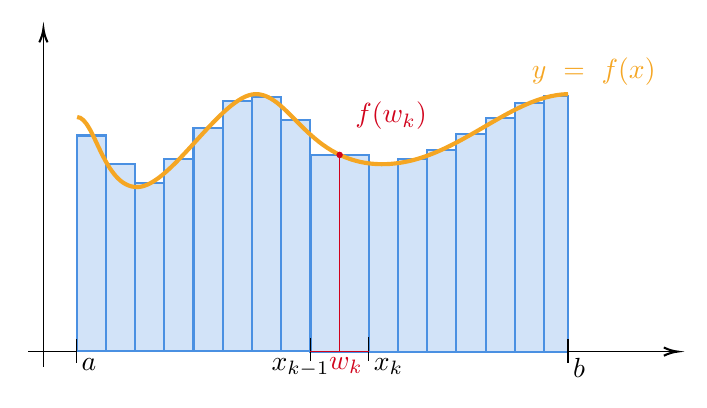
\begin{tikzpicture}[x=0.45pt,y=0.45pt,yscale=-1,xscale=1]
                %Straight Lines [id:da12841442237095768] 
                \draw    (73.88,278.15) -- (73.88,95.95) -- (73.88,8.88) ;
                \draw [shift={(73.88,6.88)}, rotate = 90] [color={rgb, 255:red, 0; green, 0; blue, 0 }  ][line width=0.75]    (10.93,-3.29) .. controls (6.95,-1.4) and (3.31,-0.3) .. (0,0) .. controls (3.31,0.3) and (6.95,1.4) .. (10.93,3.29)   ;
                %Straight Lines [id:da5483612086162443] 
                \draw    (61.67,266.16) -- (581,266.16) ;
                \draw [shift={(583,266.16)}, rotate = 180] [color={rgb, 255:red, 0; green, 0; blue, 0 }  ][line width=0.75]    (10.93,-3.29) .. controls (6.95,-1.4) and (3.31,-0.3) .. (0,0) .. controls (3.31,0.3) and (6.95,1.4) .. (10.93,3.29)   ;
                %Shape: Rectangle [id:dp44799821574678944] 
                \draw  [color={rgb, 255:red, 74; green, 144; blue, 226 }  ,draw opacity=1 ][fill={rgb, 255:red, 74; green, 144; blue, 226 }  ,fill opacity=0.25 ][line width=0.75]  (100.47,92.66) -- (123.95,92.66) -- (123.95,266.04) -- (100.47,266.04) -- cycle ;
                %Shape: Rectangle [id:dp7972527434274514] 
                \draw  [color={rgb, 255:red, 74; green, 144; blue, 226 }  ,draw opacity=1 ][fill={rgb, 255:red, 74; green, 144; blue, 226 }  ,fill opacity=0.25 ][line width=0.75]  (123.95,115.31) -- (147.42,115.31) -- (147.42,266.04) -- (123.95,266.04) -- cycle ;
                %Shape: Rectangle [id:dp35737634737767576] 
                \draw  [color={rgb, 255:red, 74; green, 144; blue, 226 }  ,draw opacity=1 ][fill={rgb, 255:red, 74; green, 144; blue, 226 }  ,fill opacity=0.25 ][line width=0.75]  (147.42,130.99) -- (170.89,130.99) -- (170.89,266.04) -- (147.42,266.04) -- cycle ;
                %Shape: Rectangle [id:dp2852872006648217] 
                \draw  [color={rgb, 255:red, 74; green, 144; blue, 226 }  ,draw opacity=1 ][fill={rgb, 255:red, 74; green, 144; blue, 226 }  ,fill opacity=0.25 ][line width=0.75]  (170.89,111.56) -- (194.37,111.56) -- (194.37,266.04) -- (170.89,266.04) -- cycle ;
                %Shape: Rectangle [id:dp9448166603081402] 
                \draw  [color={rgb, 255:red, 74; green, 144; blue, 226 }  ,draw opacity=1 ][fill={rgb, 255:red, 74; green, 144; blue, 226 }  ,fill opacity=0.25 ][line width=0.75]  (194.37,86.32) -- (217.84,86.32) -- (217.84,266.04) -- (194.37,266.04) -- cycle ;
                %Shape: Rectangle [id:dp3470258776503884] 
                \draw  [color={rgb, 255:red, 74; green, 144; blue, 226 }  ,draw opacity=1 ][fill={rgb, 255:red, 74; green, 144; blue, 226 }  ,fill opacity=0.25 ][line width=0.75]  (217.84,65.17) -- (241.32,65.17) -- (241.32,266.04) -- (217.84,266.04) -- cycle ;
                %Shape: Rectangle [id:dp41031515164445] 
                \draw  [color={rgb, 255:red, 74; green, 144; blue, 226 }  ,draw opacity=1 ][fill={rgb, 255:red, 74; green, 144; blue, 226 }  ,fill opacity=0.25 ][line width=0.75]  (241.32,61.42) -- (264.79,61.42) -- (264.79,266.04) -- (241.32,266.04) -- cycle ;
                %Shape: Rectangle [id:dp40210898491798597] 
                \draw  [color={rgb, 255:red, 74; green, 144; blue, 226 }  ,draw opacity=1 ][fill={rgb, 255:red, 74; green, 144; blue, 226 }  ,fill opacity=0.25 ][line width=0.75]  (264.79,80.52) -- (288.27,80.52) -- (288.27,266.04) -- (264.79,266.04) -- cycle ;
                %Shape: Rectangle [id:dp36980126261408597] 
                \draw  [color={rgb, 255:red, 74; green, 144; blue, 226 }  ,draw opacity=1 ][fill={rgb, 255:red, 74; green, 144; blue, 226 }  ,fill opacity=0.25 ][line width=0.75]  (288.32,108.21) -- (335.1,108.21) -- (335.1,266.16) -- (288.32,266.16) -- cycle ;
                %Shape: Rectangle [id:dp49051800646095256] 
                \draw  [color={rgb, 255:red, 74; green, 144; blue, 226 }  ,draw opacity=1 ][fill={rgb, 255:red, 74; green, 144; blue, 226 }  ,fill opacity=0.25 ][line width=0.75]  (335.1,115.66) -- (358.58,115.66) -- (358.58,266.16) -- (335.1,266.16) -- cycle ;
                %Shape: Rectangle [id:dp8466665964571507] 
                \draw  [color={rgb, 255:red, 74; green, 144; blue, 226 }  ,draw opacity=1 ][fill={rgb, 255:red, 74; green, 144; blue, 226 }  ,fill opacity=0.25 ][line width=0.75]  (358.58,111.56) -- (382.05,111.56) -- (382.05,266.16) -- (358.58,266.16) -- cycle ;
                %Shape: Rectangle [id:dp016029500323797574] 
                \draw  [color={rgb, 255:red, 74; green, 144; blue, 226 }  ,draw opacity=1 ][fill={rgb, 255:red, 74; green, 144; blue, 226 }  ,fill opacity=0.25 ][line width=0.75]  (382.05,104.39) -- (405.53,104.39) -- (405.53,266.16) -- (382.05,266.16) -- cycle ;
                %Shape: Rectangle [id:dp6213152218504514] 
                \draw  [color={rgb, 255:red, 74; green, 144; blue, 226 }  ,draw opacity=1 ][fill={rgb, 255:red, 74; green, 144; blue, 226 }  ,fill opacity=0.25 ][line width=0.75]  (405.53,91.78) -- (429,91.78) -- (429,266.16) -- (405.53,266.16) -- cycle ;
                %Shape: Rectangle [id:dp2514338685495018] 
                \draw  [color={rgb, 255:red, 74; green, 144; blue, 226 }  ,draw opacity=1 ][fill={rgb, 255:red, 74; green, 144; blue, 226 }  ,fill opacity=0.25 ][line width=0.75]  (429,78.48) -- (452.47,78.48) -- (452.47,266.16) -- (429,266.16) -- cycle ;
                %Shape: Rectangle [id:dp6055239619390653] 
                \draw  [color={rgb, 255:red, 74; green, 144; blue, 226 }  ,draw opacity=1 ][fill={rgb, 255:red, 74; green, 144; blue, 226 }  ,fill opacity=0.25 ][line width=0.75]  (452.47,66.88) -- (475.95,66.88) -- (475.95,266.16) -- (452.47,266.16) -- cycle ;
                %Shape: Rectangle [id:dp9978664781326286] 
                \draw  [color={rgb, 255:red, 74; green, 144; blue, 226 }  ,draw opacity=1 ][fill={rgb, 255:red, 74; green, 144; blue, 226 }  ,fill opacity=0.25 ][line width=0.75]  (475.95,61.08) -- (495.16,61.08) -- (495.16,266.16) -- (475.95,266.16) -- cycle ;
                %Curve Lines [id:da3818182357397808] 
                \draw [color={rgb, 255:red, 245; green, 166; blue, 35 }  ,draw opacity=1 ][line width=1.5]    (100.93,77.79) .. controls (115.06,78.11) and (121.89,134.11) .. (149.15,134.05) .. controls (176.41,133.98) and (216.92,59.39) .. (244.43,59.39) .. controls (271.94,59.39) and (287.2,115.29) .. (345.34,115.66) .. controls (403.49,116.04) and (446.39,60.5) .. (495.16,59.38) ;
                %Straight Lines [id:da09808461779354138] 
                \draw    (100.29,256.15) -- (100.29,274.91) ;
                %Straight Lines [id:da009130721014732446] 
                \draw    (495.12,256.15) -- (495.12,274.91) ;
                %Straight Lines [id:da6282232215915237] 
                \draw    (288.32,255.22) -- (288.32,273.97) ;
                %Straight Lines [id:da8799943930211327] 
                \draw    (335.22,254.75) -- (335.22,273.5) ;
                %Straight Lines [id:da3998975546032959] 
                \draw [color={rgb, 255:red, 208; green, 2; blue, 27 }  ,draw opacity=1 ]   (288.27,266.04) -- (335.22,266.04) ;
                %Straight Lines [id:da578124513030509] 
                \draw [color={rgb, 255:red, 208; green, 2; blue, 27 }  ,draw opacity=1 ]   (311.71,266.16) -- (311.71,108.21) ;
                %Shape: Ellipse [id:dp9190609134838789] 
                \draw  [color={rgb, 255:red, 208; green, 2; blue, 27 }  ,draw opacity=1 ][fill={rgb, 255:red, 208; green, 2; blue, 27 }  ,fill opacity=1 ] (309.6,108.21) .. controls (309.6,107.04) and (310.55,106.1) .. (311.71,106.1) .. controls (312.88,106.1) and (313.82,107.04) .. (313.82,108.21) .. controls (313.82,109.37) and (312.88,110.32) .. (311.71,110.32) .. controls (310.55,110.32) and (309.6,109.37) .. (309.6,108.21) -- cycle ;

                % Text Node
                \draw (463.92,27.78) node [anchor=north west][inner sep=0.75pt]    {$\textcolor[rgb]{0.96,0.65,0.14}{y\ =\ f( x)}$};
                % Text Node
                \draw (255.05,269.44) node [anchor=north west][inner sep=0.75pt]    {$x_{k-1}$};
                % Text Node
                \draw (337.1,269.56) node [anchor=north west][inner sep=0.75pt]    {$x_{k}$};
                % Text Node
                \draw (322.19,63.74) node [anchor=north west][inner sep=0.75pt]    {$\textcolor[rgb]{0.82,0.01,0.11}{f( w_{k})}$};
                % Text Node
                \draw (301.27,269.12) node [anchor=north west][inner sep=0.75pt]    {$\textcolor[rgb]{0.82,0.01,0.11}{w_{k}}$};
                % Text Node
                \draw (102.47,269.44) node [anchor=north west][inner sep=0.75pt]    {$a$};
                % Text Node
                \draw (497.16,269.56) node [anchor=north west][inner sep=0.75pt]    {$b$};
            \end{tikzpicture}
        \caption{Interpretação geométrica da integral}
        \label{fig:GeometriaIntegral}
    \end{figure}
portanto \[\int_a^b f(x) dx\] é a área sob o gráfico de \(f\) de \(a\) até \(b\).

\textbf{Pergunta: } Como podemos definir a integral para uma função de duas variáveis?

Seja \(f:D_f\subset\R^2 \to \R\) uma função e \(\mathcal{R}\subset D_f\) uma região. 

Suponha que podemos escolher uma região retângular \(\mathcal{W}\) tal que \(\mathcal{R} \subset \mathcal{W}\) da seguinte forma
    \begin{figure}[htbp]
        \centering
            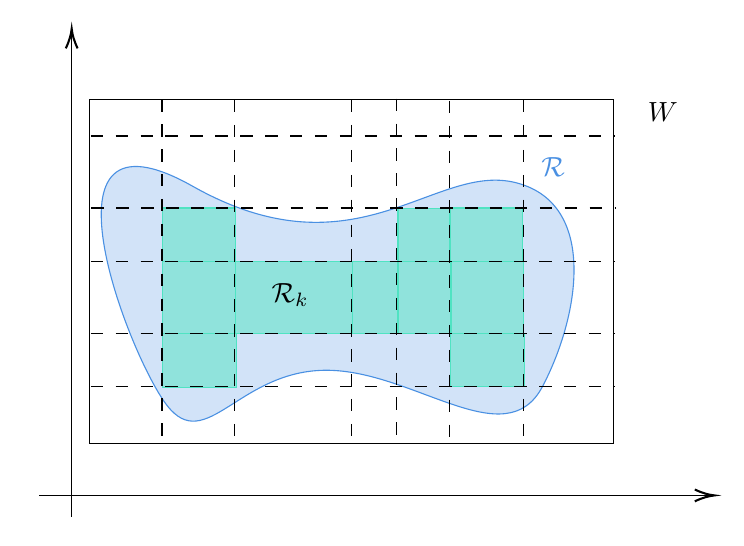
\begin{tikzpicture}[x=0.65pt,y=0.65pt,yscale=-1,xscale=1]
                %Straight Lines [id:da7864175792836353] 
                \draw    (160,281.99) -- (160,60.2) -- (160,12.55) ;
                \draw [shift={(160,10.55)}, rotate = 90] [color={rgb, 255:red, 0; green, 0; blue, 0 }  ][line width=0.75]    (10.93,-3.29) .. controls (6.95,-1.4) and (3.31,-0.3) .. (0,0) .. controls (3.31,0.3) and (6.95,1.4) .. (10.93,3.29)   ;
                %Straight Lines [id:da6176822664320704] 
                \draw    (142,270) -- (515.33,270) ;
                \draw [shift={(517.33,270)}, rotate = 180] [color={rgb, 255:red, 0; green, 0; blue, 0 }  ][line width=0.75]    (10.93,-3.29) .. controls (6.95,-1.4) and (3.31,-0.3) .. (0,0) .. controls (3.31,0.3) and (6.95,1.4) .. (10.93,3.29)   ;
                %Shape: Rectangle [id:dp7695931968927993] 
                \draw   (170,50) -- (461,50) -- (461,241) -- (170,241) -- cycle ;
                %Shape: Polygon Curved [id:ds9573654547058211] 
                \draw  [color={rgb, 255:red, 74; green, 144; blue, 226 }  ,draw opacity=1 ][fill={rgb, 255:red, 74; green, 144; blue, 226 }  ,fill opacity=0.25 ] (227.18,98.08) .. controls (318.52,149.61) and (361.51,84.47) .. (407.11,96.19) .. controls (452.71,107.92) and (442.29,170.45) .. (421.73,209.46) .. controls (401.17,248.47) and (350.22,200.42) .. (301.58,200.42) .. controls (252.95,200.42) and (234.61,247.8) .. (212.99,219.96) .. controls (191.38,192.11) and (135.84,46.56) .. (227.18,98.08) -- cycle ;
                %Shape: Rectangle [id:dp6041179300175292] 
                \draw  [color={rgb, 255:red, 80; green, 227; blue, 194 }  ,draw opacity=1 ][fill={rgb, 255:red, 80; green, 227; blue, 194 }  ,fill opacity=0.5 ] (210.4,110.2) -- (251,110.2) -- (251,140.2) -- (210.4,140.2) -- cycle ;
                %Shape: Rectangle [id:dp25634125667822905] 
                \draw  [color={rgb, 255:red, 80; green, 227; blue, 194 }  ,draw opacity=1 ][fill={rgb, 255:red, 80; green, 227; blue, 194 }  ,fill opacity=0.5 ] (210.4,140.2) -- (251,140.2) -- (251,180.2) -- (210.4,180.2) -- cycle ;
                %Shape: Rectangle [id:dp24956429410548986] 
                \draw  [color={rgb, 255:red, 80; green, 227; blue, 194 }  ,draw opacity=1 ][fill={rgb, 255:red, 80; green, 227; blue, 194 }  ,fill opacity=0.5 ] (251,140.2) -- (316.2,140.2) -- (316.2,180.2) -- (251,180.2) -- cycle ;
                %Shape: Rectangle [id:dp5850691653276779] 
                \draw  [color={rgb, 255:red, 80; green, 227; blue, 194 }  ,draw opacity=1 ][fill={rgb, 255:red, 80; green, 227; blue, 194 }  ,fill opacity=0.5 ] (210.4,180.2) -- (251.4,180.2) -- (251.4,209.8) -- (210.4,209.8) -- cycle ;
                %Shape: Rectangle [id:dp020812649152888163] 
                \draw  [color={rgb, 255:red, 80; green, 227; blue, 194 }  ,draw opacity=1 ][fill={rgb, 255:red, 80; green, 227; blue, 194 }  ,fill opacity=0.5 ] (316.2,140.2) -- (341.4,140.2) -- (341.4,180.2) -- (316.2,180.2) -- cycle ;
                %Shape: Rectangle [id:dp006904193515761214] 
                \draw  [color={rgb, 255:red, 80; green, 227; blue, 194 }  ,draw opacity=1 ][fill={rgb, 255:red, 80; green, 227; blue, 194 }  ,fill opacity=0.5 ] (341.4,110.6) -- (370.6,110.6) -- (370.6,139.8) -- (341.4,139.8) -- cycle ;
                %Shape: Rectangle [id:dp12103193668807266] 
                \draw  [color={rgb, 255:red, 80; green, 227; blue, 194 }  ,draw opacity=1 ][fill={rgb, 255:red, 80; green, 227; blue, 194 }  ,fill opacity=0.5 ] (370.2,110.2) -- (410.6,110.2) -- (410.6,139.8) -- (370.2,139.8) -- cycle ;
                %Shape: Rectangle [id:dp9548528325145071] 
                \draw  [color={rgb, 255:red, 80; green, 227; blue, 194 }  ,draw opacity=1 ][fill={rgb, 255:red, 80; green, 227; blue, 194 }  ,fill opacity=0.5 ] (341.4,139.8) -- (371,139.8) -- (371,179.8) -- (341.4,179.8) -- cycle ;
                %Shape: Rectangle [id:dp9275534408738052] 
                \draw  [color={rgb, 255:red, 80; green, 227; blue, 194 }  ,draw opacity=1 ][fill={rgb, 255:red, 80; green, 227; blue, 194 }  ,fill opacity=0.5 ] (370.6,139.8) -- (411.4,139.8) -- (411.4,179.8) -- (370.6,179.8) -- cycle ;
                %Shape: Rectangle [id:dp8049033090850595] 
                \draw  [color={rgb, 255:red, 80; green, 227; blue, 194 }  ,draw opacity=1 ][fill={rgb, 255:red, 80; green, 227; blue, 194 }  ,fill opacity=0.5 ] (370.6,179.8) -- (411.8,179.8) -- (411.8,209.4) -- (370.6,209.4) -- cycle ;
                %Straight Lines [id:da07519315148872174] 
                \draw  [dash pattern={on 4.5pt off 4.5pt}]  (170.6,70.2) -- (461.4,70.2) ;
                %Straight Lines [id:da9127778140313066] 
                \draw  [dash pattern={on 4.5pt off 4.5pt}]  (171,110.2) -- (461.8,110.2) ;
                %Straight Lines [id:da30227104311369835] 
                \draw  [dash pattern={on 4.5pt off 4.5pt}]  (170.6,139.8) -- (461.4,139.8) ;
                %Straight Lines [id:da9984810321408175] 
                \draw  [dash pattern={on 4.5pt off 4.5pt}]  (170.6,179.8) -- (461.4,179.8) ;
                %Straight Lines [id:da6031310780324549] 
                \draw  [dash pattern={on 4.5pt off 4.5pt}]  (170.6,209.4) -- (461.4,209.4) ;
                %Straight Lines [id:da9841151805678033] 
                \draw  [dash pattern={on 4.5pt off 4.5pt}]  (210.2,49.8) -- (210.2,240.6) ;
                %Straight Lines [id:da9267445252169808] 
                \draw  [dash pattern={on 4.5pt off 4.5pt}]  (250.6,50.2) -- (250.6,241) ;
                %Straight Lines [id:da6432124554722044] 
                \draw  [dash pattern={on 4.5pt off 4.5pt}]  (315.5,50.2) -- (315.5,241) ;
                %Straight Lines [id:da8892025464829473] 
                \draw  [dash pattern={on 4.5pt off 4.5pt}]  (340.6,49.4) -- (340.6,240.2) ;
                %Straight Lines [id:da21494557275083181] 
                \draw  [dash pattern={on 4.5pt off 4.5pt}]  (370.2,50.6) -- (370.2,241.4) ;
                %Straight Lines [id:da18419319627522945] 
                \draw  [dash pattern={on 4.5pt off 4.5pt}]  (411,50.2) -- (411,241) ;

                % Text Node
                \draw (419.71,80.52) node [anchor=north west][inner sep=0.75pt]  [color={rgb, 255:red, 74; green, 144; blue, 226 }  ,opacity=1 ]  {$\mathcal{R}$};
                % Text Node
                \draw (478.89,50.16) node [anchor=north west][inner sep=0.75pt]    {$W$};
                % Text Node
                \draw (269.71,150.92) node [anchor=north west][inner sep=0.75pt]  [color={rgb, 255:red, 0; green, 0; blue, 0 }  ,opacity=1 ]  {$\mathcal{R}_{k}$};
            \end{tikzpicture}
        \caption{Região \(\mathcal{W}\)}
        \label{fig:Malha}
    \end{figure}

\begin{definition}
    Se \(\mathcal{W}\) é dividida em retângulos por meio de uma rede de retas horizontais e verticais, então o conjunto de todos os retângulos completamente contidos em \(\mathcal{R}\) se chama \textbf{partição interior}\index{Partição! Interior} de \(\mathcal{R}\)
\end{definition}

\begin{definition}
    Seja \(P_n = \{\mathcal{R}_1, \mathcal{R}_2, \dots, \mathcal{R}_n\}\) uma partição interior de \(\mathcal{R}\). Denotamos por \(\Delta A_k\) a área de \(\mathcal{R}_k\). Além disso, o comprimento da maior diagonal de todos os \(\mathcal{R}_k\) é a \textbf{norma} \(\|P_n\|\) da partição \(P_n\).
\end{definition}

\begin{definition}
    Uma \textbf{soma de Riemann}\index{Soma de Riemann} de \(f\) para uma partição \(P_n\) é dada por \[S(P_n) = \sum_{k=1}^{n} f(u_k,v_k)\cdot \Delta A_k,\] no qual \((u_k,v_k)\in\mathcal{R}_k\) é um ponto arbitrário.
\end{definition}

\begin{definition}
    A \textbf{integral dupla}\index{Integral dupla} de \(f\) em \(\mathcal{R}\) é definida como \[\int\int_\mathcal{R} f(x,y) dA = \lim_{\|P_n\| \to 0} \sum_{k=1}^{n} f(u_k,v_k)\cdot\Delta A_k,\] desde que o limite exista.
\end{definition}

Em outras palavras, dado \(\varepsilon > 0\), existe \(\delta>0\) tal que se \(\|P_n\| < \delta\), então \[\left| \sum_{k=1}^{n} f(u_k,v_k)\cdot\Delta A_k - \int\int_\mathcal{R} f(x,y) dA\right| < \varepsilon.\] Neste caso, dizemos que \(f\) é \textit{integrável} sobre \(\mathcal{R}\).

\begin{remark}
    Podemos provar que se \(f\) é contínua em \(\mathcal{R}\), então \(f\) é integrável em \(\mathcal{R}\).
\end{remark}

\subsection{Interpretação geométrica da integral dupla}

Seja \(f: D_f\subset\R^2 \to \R\) uma função contínua tal que \(f(x,y)\geq 0\) numa região \(\mathcal{R}\).

Se
    \begin{itemize}
        \item \(S\) é o gráfico de \(f\),
        \item \(Q\) é o sólido abaixo de \(S\) e acima de \(\mathcal{R}\),
        \item e \((u_k,v_k)\in\mathcal{R}_k\)
    \end{itemize}
        \begin{figure}[htbp]
            \centering
            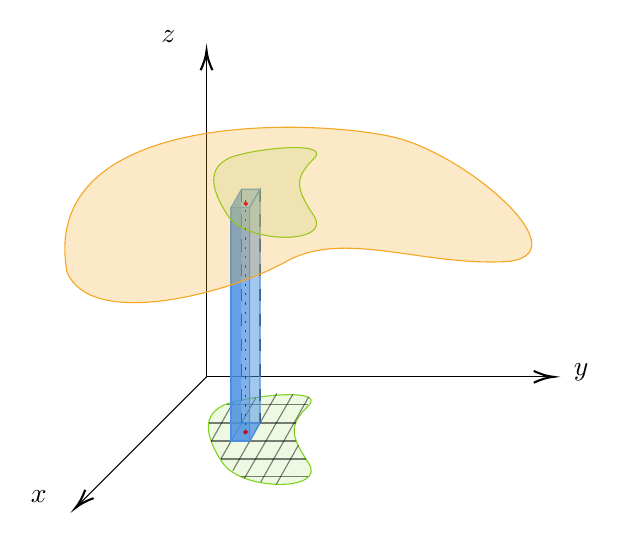
\begin{tikzpicture}[x=0.65pt,y=0.65pt,yscale=-1,xscale=1]
            %Straight Lines [id:da4417917463521195] 
                \draw    (125,214.58) -- (125,35.16) ;
                \draw [shift={(125,33.16)}, rotate = 90] [color={rgb, 255:red, 0; green, 0; blue, 0 }  ][line width=0.75]    (10.93,-3.29) .. controls (6.95,-1.4) and (3.31,-0.3) .. (0,0) .. controls (3.31,0.3) and (6.95,1.4) .. (10.93,3.29)   ;
                %Straight Lines [id:da2972891010842106] 
                \draw    (125,214.58) -- (315.83,214.58) ;
                \draw [shift={(317.83,214.58)}, rotate = 180] [color={rgb, 255:red, 0; green, 0; blue, 0 }  ][line width=0.75]    (10.93,-3.29) .. controls (6.95,-1.4) and (3.31,-0.3) .. (0,0) .. controls (3.31,0.3) and (6.95,1.4) .. (10.93,3.29)   ;
                %Straight Lines [id:da10972918853050884] 
                \draw    (125,214.58) -- (53.55,286.04) ;
                \draw [shift={(52.13,287.45)}, rotate = 315] [color={rgb, 255:red, 0; green, 0; blue, 0 }  ][line width=0.75]    (10.93,-3.29) .. controls (6.95,-1.4) and (3.31,-0.3) .. (0,0) .. controls (3.31,0.3) and (6.95,1.4) .. (10.93,3.29)   ;
                %Shape: Regular Polygon [id:dp4300554733979206] 
                \draw  [color={rgb, 255:red, 126; green, 211; blue, 33 }  ,draw opacity=1 ][fill={rgb, 255:red, 184; green, 233; blue, 134 }  ,fill opacity=0.25 ] (133.95,230.62) .. controls (144.56,225.32) and (192.28,220.02) .. (181.67,230.62) .. controls (171.07,241.23) and (171.07,246.53) .. (181.67,262.44) .. controls (192.28,278.34) and (144.56,278.34) .. (133.95,262.44) .. controls (123.35,246.53) and (123.35,235.92) .. (133.95,230.62) -- cycle ;
                %Straight Lines [id:da734870218783715] 
                \draw [color={rgb, 255:red, 0; green, 0; blue, 0 }  ,draw opacity=0.5 ]   (140.04,228.36) -- (127.73,250.23) ;
                %Straight Lines [id:da6385554597781345] 
                \draw [color={rgb, 255:red, 0; green, 0; blue, 0 }  ,draw opacity=0.5 ]   (152.4,226.23) -- (132.98,260.23) ;
                %Straight Lines [id:da1465213241031078] 
                \draw [color={rgb, 255:red, 0; green, 0; blue, 0 }  ,draw opacity=0.5 ]   (164.1,223.73) -- (139.6,266.8) ;
                %Straight Lines [id:da9525764107579172] 
                \draw [color={rgb, 255:red, 0; green, 0; blue, 0 }  ,draw opacity=0.5 ]   (172.93,224.36) -- (146.04,271.02) ;
                %Straight Lines [id:da7895350785159607] 
                \draw [color={rgb, 255:red, 0; green, 0; blue, 0 }  ,draw opacity=0.5 ]   (181.82,225.69) -- (155.16,273.02) ;
                %Straight Lines [id:da946873877220359] 
                \draw [color={rgb, 255:red, 0; green, 0; blue, 0 }  ,draw opacity=0.5 ]   (136.23,229.98) -- (181.67,229.98) ;
                %Straight Lines [id:da13138180503164054] 
                \draw [color={rgb, 255:red, 0; green, 0; blue, 0 }  ,draw opacity=0.5 ]   (126.23,240.23) -- (174.5,240.23) ;
                %Straight Lines [id:da8256661881519005] 
                \draw [color={rgb, 255:red, 0; green, 0; blue, 0 }  ,draw opacity=0.5 ]   (127.73,250.23) -- (175,250.23) ;
                %Straight Lines [id:da4825477345227942] 
                \draw [color={rgb, 255:red, 0; green, 0; blue, 0 }  ,draw opacity=0.5 ]   (132.98,260.23) -- (180.25,260.23) ;
                %Straight Lines [id:da3951095172947672] 
                \draw [color={rgb, 255:red, 0; green, 0; blue, 0 }  ,draw opacity=0.5 ]   (143.98,269.98) -- (181.5,269.98) ;
                %Straight Lines [id:da42102236749069266] 
                \draw [color={rgb, 255:red, 0; green, 0; blue, 0 }  ,draw opacity=0.5 ]   (176.04,252.58) -- (163.73,274.45) ;
                %Shape: Rectangle [id:dp6150229131744026] 
                \draw  [color={rgb, 255:red, 74; green, 144; blue, 226 }  ,draw opacity=1 ][fill={rgb, 255:red, 74; green, 144; blue, 226 }  ,fill opacity=0.5 ] (144.41,240.23) -- (154.72,240.23) -- (148.93,250.36) -- (138.62,250.36) -- cycle ;
                %Straight Lines [id:da7380067554299922] 
                \draw [color={rgb, 255:red, 74; green, 144; blue, 226 }  ,draw opacity=1 ]   (138.62,120.43) -- (138.62,250.36) ;
                %Straight Lines [id:da34613782229176593] 
                \draw    (148.93,120.43) -- (148.93,250.36) ;
                %Straight Lines [id:da8565316842715038] 
                \draw  [dash pattern={on 4.5pt off 4.5pt}]  (144.41,110.31) -- (144.41,240.23) ;
                %Straight Lines [id:da21133650245427738] 
                \draw  [dash pattern={on 4.5pt off 4.5pt}]  (154.72,110.31) -- (154.72,240.23) ;
                %Shape: Rectangle [id:dp4446163243637161] 
                \draw  [color={rgb, 255:red, 74; green, 144; blue, 226 }  ,draw opacity=1 ][fill={rgb, 255:red, 74; green, 144; blue, 226 }  ,fill opacity=0.5 ] (144.41,110.31) -- (154.72,110.31) -- (148.93,120.43) -- (138.62,120.43) -- cycle ;
                %Shape: Polygon [id:ds5027928984310592] 
                \draw  [color={rgb, 255:red, 74; green, 144; blue, 226 }  ,draw opacity=1 ][fill={rgb, 255:red, 74; green, 144; blue, 226 }  ,fill opacity=0.5 ] (154.72,110.31) -- (154.72,240.23) -- (148.93,250.36) -- (148.93,120.43) -- cycle ;
                %Shape: Polygon [id:ds8331426858272624] 
                \draw  [draw opacity=0][fill={rgb, 255:red, 74; green, 144; blue, 226 }  ,fill opacity=0.5 ] (144.41,110.31) -- (144.41,240.23) -- (138.62,250.36) -- (138.62,120.43) -- cycle ;
                %Shape: Polygon [id:ds11523874573891169] 
                \draw  [draw opacity=0][fill={rgb, 255:red, 74; green, 144; blue, 226 }  ,fill opacity=0.7 ] (138.62,120.43) -- (148.93,120.43) -- (148.93,250.36) -- (138.62,250.36) -- cycle ;
                %Shape: Regular Polygon [id:dp2751964050819099] 
                \draw  [color={rgb, 255:red, 126; green, 211; blue, 33 }  ,draw opacity=1 ][fill={rgb, 255:red, 184; green, 233; blue, 134 }  ,fill opacity=0.25 ] (136.95,93.26) .. controls (147.56,87.95) and (195.28,82.65) .. (184.67,93.26) .. controls (174.07,103.86) and (174.07,109.16) .. (184.67,125.07) .. controls (195.28,140.98) and (147.56,140.98) .. (136.95,125.07) .. controls (126.35,109.16) and (126.35,98.56) .. (136.95,93.26) -- cycle ;
                %Shape: Circle [id:dp08554144399628916] 
                \draw  [color={rgb, 255:red, 208; green, 2; blue, 27 }  ,draw opacity=1 ][fill={rgb, 255:red, 208; green, 2; blue, 27 }  ,fill opacity=1 ] (145.67,245.29) .. controls (145.67,244.74) and (146.12,244.29) .. (146.67,244.29) .. controls (147.22,244.29) and (147.67,244.74) .. (147.67,245.29) .. controls (147.67,245.84) and (147.22,246.29) .. (146.67,246.29) .. controls (146.12,246.29) and (145.67,245.84) .. (145.67,245.29) -- cycle ;
                %Straight Lines [id:da3484479168201685] 
                \draw [color={rgb, 255:red, 208; green, 2; blue, 27 }  ,draw opacity=1 ] [dash pattern={on 0.84pt off 2.51pt}]  (146.71,116.44) -- (146.71,244.34) ;
                %Shape: Circle [id:dp6747429045839405] 
                \draw  [color={rgb, 255:red, 208; green, 2; blue, 27 }  ,draw opacity=1 ][fill={rgb, 255:red, 208; green, 2; blue, 27 }  ,fill opacity=1 ] (145.82,118.32) .. controls (145.82,117.77) and (146.27,117.32) .. (146.83,117.32) .. controls (147.38,117.32) and (147.83,117.77) .. (147.83,118.32) .. controls (147.83,118.88) and (147.38,119.32) .. (146.83,119.32) .. controls (146.27,119.32) and (145.82,118.88) .. (145.82,118.32) -- cycle ;
                %Curve Lines [id:da9211510542299556] 
                \draw [color={rgb, 255:red, 245; green, 166; blue, 35 }  ,draw opacity=1 ][fill={rgb, 255:red, 245; green, 166; blue, 35 }  ,fill opacity=0.25 ]   (47.38,156.14) .. controls (31.2,64.5) and (188.35,71.37) .. (229.81,81.51) .. controls (271.27,91.64) and (336.2,148.72) .. (289.7,150.61) .. controls (243.2,152.5) and (200.8,132.72) .. (169,150.61) .. controls (137.2,168.5) and (60.2,188.5) .. (47.38,156.14) -- cycle ;

                % Text Node
                \draw (25.87,276.38) node [anchor=north west][inner sep=0.75pt]  [font=\normalsize]  {$x$};
                % Text Node
                \draw (98.43,20.78) node [anchor=north west][inner sep=0.75pt]  [font=\normalsize]  {$z$};
                % Text Node
                \draw (327.7,205.67) node [anchor=north west][inner sep=0.75pt]  [font=\normalsize]  {$y$};
            \end{tikzpicture}
            \caption{Volume do prisma de base retangular \(\mathcal{R}_k\) e altura \(f(u_k,v_k)\)}
            \label{fig:VolumePrisma}
        \end{figure}
Então, \(f(u_k,v_k)\cdot\Delta A_k\) é o volume do prisma de base retangular de área \(\Lambda A_k\) e altura \(f(u_k,v_k)\).

A soma de todos esses volumes de prismas é uma \textit{aproximação} do volume \(V\) de \(Q\), que melhora quando \(\|P_n\|\to 0\), ou seja, quando temos \(\mathcal{R}_k\) cada vez menores.
        \begin{figure}[htbp]
            \centering
            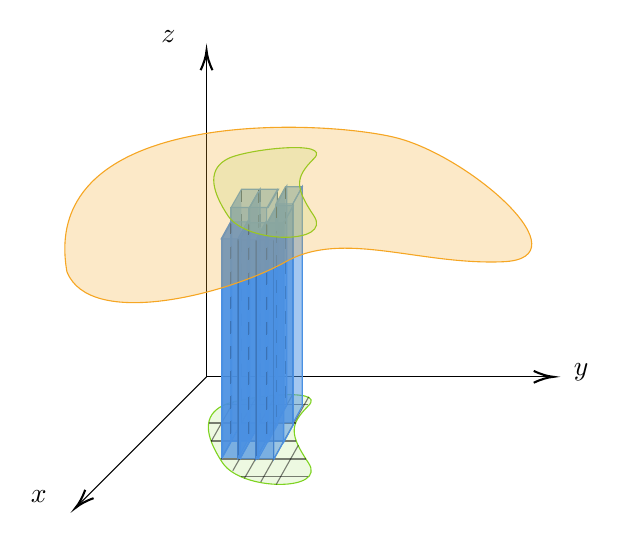
\begin{tikzpicture}[x=0.65pt,y=0.65pt,yscale=-1,xscale=1]
                %Straight Lines [id:da7301665929090642] 
                \draw    (125,214.58) -- (125,35.16) ;
                \draw [shift={(125,33.16)}, rotate = 90] [color={rgb, 255:red, 0; green, 0; blue, 0 }  ][line width=0.75]    (10.93,-3.29) .. controls (6.95,-1.4) and (3.31,-0.3) .. (0,0) .. controls (3.31,0.3) and (6.95,1.4) .. (10.93,3.29)   ;
                %Straight Lines [id:da4027073420421289] 
                \draw    (125,214.58) -- (315.83,214.58) ;
                \draw [shift={(317.83,214.58)}, rotate = 180] [color={rgb, 255:red, 0; green, 0; blue, 0 }  ][line width=0.75]    (10.93,-3.29) .. controls (6.95,-1.4) and (3.31,-0.3) .. (0,0) .. controls (3.31,0.3) and (6.95,1.4) .. (10.93,3.29)   ;
                %Straight Lines [id:da12189966807540975] 
                \draw    (125,214.58) -- (53.55,286.04) ;
                \draw [shift={(52.13,287.45)}, rotate = 315] [color={rgb, 255:red, 0; green, 0; blue, 0 }  ][line width=0.75]    (10.93,-3.29) .. controls (6.95,-1.4) and (3.31,-0.3) .. (0,0) .. controls (3.31,0.3) and (6.95,1.4) .. (10.93,3.29)   ;
                %Shape: Regular Polygon [id:dp7501792077910774] 
                \draw  [color={rgb, 255:red, 126; green, 211; blue, 33 }  ,draw opacity=1 ][fill={rgb, 255:red, 184; green, 233; blue, 134 }  ,fill opacity=0.25 ] (133.95,230.62) .. controls (144.56,225.32) and (192.28,220.02) .. (181.67,230.62) .. controls (171.07,241.23) and (171.07,246.53) .. (181.67,262.44) .. controls (192.28,278.34) and (144.56,278.34) .. (133.95,262.44) .. controls (123.35,246.53) and (123.35,235.92) .. (133.95,230.62) -- cycle ;
                %Straight Lines [id:da10051099221045456] 
                \draw [color={rgb, 255:red, 0; green, 0; blue, 0 }  ,draw opacity=0.5 ]   (140.04,228.36) -- (127.73,250.23) ;
                %Straight Lines [id:da5912483427676196] 
                \draw [color={rgb, 255:red, 0; green, 0; blue, 0 }  ,draw opacity=0.5 ]   (152.4,226.23) -- (132.98,260.23) ;
                %Straight Lines [id:da679113758427642] 
                \draw [color={rgb, 255:red, 0; green, 0; blue, 0 }  ,draw opacity=0.5 ]   (164.1,223.73) -- (139.6,266.8) ;
                %Straight Lines [id:da415997882014129] 
                \draw [color={rgb, 255:red, 0; green, 0; blue, 0 }  ,draw opacity=0.5 ]   (172.93,224.36) -- (146.04,271.02) ;
                %Straight Lines [id:da6260584722031874] 
                \draw [color={rgb, 255:red, 0; green, 0; blue, 0 }  ,draw opacity=0.5 ]   (181.82,225.69) -- (155.16,273.02) ;
                %Straight Lines [id:da3087488799389838] 
                \draw [color={rgb, 255:red, 0; green, 0; blue, 0 }  ,draw opacity=0.5 ]   (136.23,229.98) -- (181.67,229.98) ;
                %Straight Lines [id:da4727427862351784] 
                \draw [color={rgb, 255:red, 0; green, 0; blue, 0 }  ,draw opacity=0.5 ]   (126.23,240.23) -- (174.5,240.23) ;
                %Straight Lines [id:da8475503038473085] 
                \draw [color={rgb, 255:red, 0; green, 0; blue, 0 }  ,draw opacity=0.5 ]   (127.73,250.23) -- (175,250.23) ;
                %Straight Lines [id:da40184130064260803] 
                \draw [color={rgb, 255:red, 0; green, 0; blue, 0 }  ,draw opacity=0.5 ]   (132.98,260.23) -- (180.25,260.23) ;
                %Straight Lines [id:da31172453720536053] 
                \draw [color={rgb, 255:red, 0; green, 0; blue, 0 }  ,draw opacity=0.5 ]   (143.98,269.98) -- (181.5,269.98) ;
                %Straight Lines [id:da7623174109659672] 
                \draw [color={rgb, 255:red, 0; green, 0; blue, 0 }  ,draw opacity=0.5 ]   (176.04,252.58) -- (163.73,274.45) ;
                %Shape: Rectangle [id:dp5031679700076116] 
                \draw  [color={rgb, 255:red, 74; green, 144; blue, 226 }  ,draw opacity=1 ][fill={rgb, 255:red, 74; green, 144; blue, 226 }  ,fill opacity=0.5 ] (144.41,240.23) -- (154.72,240.23) -- (148.93,250.36) -- (138.62,250.36) -- cycle ;
                %Straight Lines [id:da798993386227191] 
                \draw [color={rgb, 255:red, 74; green, 144; blue, 226 }  ,draw opacity=1 ]   (138.62,120.43) -- (138.62,250.36) ;
                %Straight Lines [id:da9375876710613786] 
                \draw    (148.93,120.43) -- (148.93,250.36) ;
                %Straight Lines [id:da9521903616711812] 
                \draw  [dash pattern={on 4.5pt off 4.5pt}]  (144.41,110.31) -- (144.41,240.23) ;
                %Straight Lines [id:da42253596107594826] 
                \draw  [dash pattern={on 4.5pt off 4.5pt}]  (154.72,110.31) -- (154.72,240.23) ;
                %Shape: Rectangle [id:dp6594158336491123] 
                \draw  [color={rgb, 255:red, 74; green, 144; blue, 226 }  ,draw opacity=1 ][fill={rgb, 255:red, 74; green, 144; blue, 226 }  ,fill opacity=0.5 ] (144.41,110.31) -- (154.72,110.31) -- (148.93,120.43) -- (138.62,120.43) -- cycle ;
                %Shape: Polygon [id:ds7799126222912717] 
                \draw  [color={rgb, 255:red, 74; green, 144; blue, 226 }  ,draw opacity=1 ][fill={rgb, 255:red, 74; green, 144; blue, 226 }  ,fill opacity=0.5 ] (154.72,110.31) -- (154.72,240.23) -- (148.93,250.36) -- (148.93,120.43) -- cycle ;
                %Shape: Polygon [id:ds807972207893949] 
                \draw  [draw opacity=0][fill={rgb, 255:red, 74; green, 144; blue, 226 }  ,fill opacity=0.5 ] (144.41,110.31) -- (144.41,240.23) -- (138.62,250.36) -- (138.62,120.43) -- cycle ;
                %Shape: Polygon [id:ds2888276628511651] 
                \draw  [draw opacity=0][fill={rgb, 255:red, 74; green, 144; blue, 226 }  ,fill opacity=0.7 ] (138.62,120.43) -- (148.93,120.43) -- (148.93,250.36) -- (138.62,250.36) -- cycle ;
                %Straight Lines [id:da0069539187483976805] 
                \draw [color={rgb, 255:red, 74; green, 144; blue, 226 }  ,draw opacity=1 ]   (148.12,120.93) -- (148.12,250.86) ;
                %Straight Lines [id:da5778771065565323] 
                \draw    (158.43,120.93) -- (158.43,250.86) ;
                %Straight Lines [id:da7787390568337622] 
                \draw  [dash pattern={on 4.5pt off 4.5pt}]  (153.91,110.81) -- (153.91,240.73) ;
                %Straight Lines [id:da7218253791420043] 
                \draw  [dash pattern={on 4.5pt off 4.5pt}]  (164.22,110.81) -- (164.22,240.73) ;
                %Shape: Polygon [id:ds7648021056962186] 
                \draw  [color={rgb, 255:red, 74; green, 144; blue, 226 }  ,draw opacity=1 ][fill={rgb, 255:red, 74; green, 144; blue, 226 }  ,fill opacity=0.5 ] (164.22,110.81) -- (164.22,240.73) -- (158.43,250.86) -- (158.43,120.93) -- cycle ;
                %Shape: Polygon [id:ds39515980536243134] 
                \draw  [draw opacity=0][fill={rgb, 255:red, 74; green, 144; blue, 226 }  ,fill opacity=0.5 ] (153.91,110.81) -- (153.91,240.73) -- (148.12,250.86) -- (148.12,120.93) -- cycle ;
                %Shape: Polygon [id:ds8215130357596798] 
                \draw  [draw opacity=0][fill={rgb, 255:red, 74; green, 144; blue, 226 }  ,fill opacity=0.7 ] (148.12,120.93) -- (158.43,120.93) -- (158.43,250.86) -- (148.12,250.86) -- cycle ;
                %Shape: Rectangle [id:dp4686184687882866] 
                \draw  [color={rgb, 255:red, 74; green, 144; blue, 226 }  ,draw opacity=1 ][fill={rgb, 255:red, 74; green, 144; blue, 226 }  ,fill opacity=0.5 ] (154.72,110.31) -- (165.03,110.31) -- (159.25,120.43) -- (148.93,120.43) -- cycle ;
                %Straight Lines [id:da36458116431746157] 
                \draw    (133.86,137.45) -- (133.86,259.39) ;
                %Straight Lines [id:da9807754723115738] 
                \draw  [dash pattern={on 4.5pt off 4.5pt}]  (139.1,127.95) -- (139.1,249.88) ;
                %Shape: Polygon [id:ds1054900048682379] 
                \draw  [color={rgb, 255:red, 74; green, 144; blue, 226 }  ,draw opacity=1 ][fill={rgb, 255:red, 74; green, 144; blue, 226 }  ,fill opacity=0.5 ] (139.1,127.95) -- (139.1,249.88) -- (133.86,259.39) -- (133.86,137.45) -- cycle ;
                %Straight Lines [id:da11235446650547554] 
                \draw [color={rgb, 255:red, 74; green, 144; blue, 226 }  ,draw opacity=1 ]   (133.12,137.92) -- (133.12,259.86) ;
                %Straight Lines [id:da9267173541244453] 
                \draw    (142.47,137.92) -- (142.47,259.86) ;
                %Straight Lines [id:da3823759023317783] 
                \draw  [dash pattern={on 4.5pt off 4.5pt}]  (138.37,128.42) -- (138.37,250.35) ;
                %Straight Lines [id:da09500590199733117] 
                \draw  [dash pattern={on 4.5pt off 4.5pt}]  (147.71,128.42) -- (147.71,250.35) ;
                %Shape: Polygon [id:ds27945353975272635] 
                \draw  [color={rgb, 255:red, 74; green, 144; blue, 226 }  ,draw opacity=1 ][fill={rgb, 255:red, 74; green, 144; blue, 226 }  ,fill opacity=0.5 ] (147.71,128.42) -- (147.71,250.35) -- (142.47,259.86) -- (142.47,137.92) -- cycle ;
                %Shape: Polygon [id:ds41489848603226376] 
                \draw  [draw opacity=0][fill={rgb, 255:red, 74; green, 144; blue, 226 }  ,fill opacity=0.5 ] (138.37,128.42) -- (138.37,250.35) -- (133.12,259.86) -- (133.12,137.92) -- cycle ;
                %Shape: Polygon [id:ds8190834534921736] 
                \draw  [draw opacity=0][fill={rgb, 255:red, 74; green, 144; blue, 226 }  ,fill opacity=0.7 ] (133.12,137.92) -- (142.47,137.92) -- (142.47,259.86) -- (133.12,259.86) -- cycle ;
                %Shape: Rectangle [id:dp6553365245012972] 
                \draw  [color={rgb, 255:red, 74; green, 144; blue, 226 }  ,draw opacity=1 ][fill={rgb, 255:red, 74; green, 144; blue, 226 }  ,fill opacity=0.5 ] (138.37,128.42) -- (147.71,128.42) -- (142.47,137.92) -- (133.12,137.92) -- cycle ;

                %Straight Lines [id:da37740756482839377] 
                \draw    (164.36,117.95) -- (164.36,239.89) ;
                %Straight Lines [id:da8032141625683007] 
                \draw  [dash pattern={on 4.5pt off 4.5pt}]  (169.6,108.45) -- (169.6,230.38) ;
                %Shape: Polygon [id:ds7935992700537446] 
                \draw  [color={rgb, 255:red, 74; green, 144; blue, 226 }  ,draw opacity=1 ][fill={rgb, 255:red, 74; green, 144; blue, 226 }  ,fill opacity=0.5 ] (169.6,108.45) -- (169.6,230.38) -- (164.36,239.89) -- (164.36,117.95) -- cycle ;
                %Straight Lines [id:da7402725998477633] 
                \draw [color={rgb, 255:red, 74; green, 144; blue, 226 }  ,draw opacity=1 ]   (163.62,118.42) -- (163.62,240.36) ;
                %Straight Lines [id:da7571219323819255] 
                \draw    (172.97,118.42) -- (172.97,240.36) ;
                %Straight Lines [id:da6603697668612233] 
                \draw  [dash pattern={on 4.5pt off 4.5pt}]  (168.87,108.92) -- (168.87,230.85) ;
                %Straight Lines [id:da6817319425952285] 
                \draw  [dash pattern={on 4.5pt off 4.5pt}]  (178.21,108.92) -- (178.21,230.85) ;
                %Shape: Polygon [id:ds7868616037785564] 
                \draw  [color={rgb, 255:red, 74; green, 144; blue, 226 }  ,draw opacity=1 ][fill={rgb, 255:red, 74; green, 144; blue, 226 }  ,fill opacity=0.5 ] (178.21,108.92) -- (178.21,230.85) -- (172.97,240.36) -- (172.97,118.42) -- cycle ;
                %Shape: Polygon [id:ds13182198676645362] 
                \draw  [draw opacity=0][fill={rgb, 255:red, 74; green, 144; blue, 226 }  ,fill opacity=0.5 ] (168.87,108.92) -- (168.87,230.85) -- (163.62,240.36) -- (163.62,118.42) -- cycle ;
                %Shape: Polygon [id:ds7945653635876782] 
                \draw  [draw opacity=0][fill={rgb, 255:red, 74; green, 144; blue, 226 }  ,fill opacity=0.7 ] (163.62,118.42) -- (172.97,118.42) -- (172.97,240.36) -- (163.62,240.36) -- cycle ;
                %Shape: Rectangle [id:dp6511878367528602] 
                \draw  [color={rgb, 255:red, 74; green, 144; blue, 226 }  ,draw opacity=1 ][fill={rgb, 255:red, 74; green, 144; blue, 226 }  ,fill opacity=0.5 ] (168.87,108.92) -- (178.21,108.92) -- (172.97,118.42) -- (163.62,118.42) -- cycle ;

                %Straight Lines [id:da25546817267584043] 
                \draw    (143.86,137.95) -- (143.86,259.89) ;
                %Straight Lines [id:da749085000924693] 
                \draw  [dash pattern={on 4.5pt off 4.5pt}]  (149.1,128.45) -- (149.1,250.38) ;
                %Shape: Polygon [id:ds638759326819409] 
                \draw  [color={rgb, 255:red, 74; green, 144; blue, 226 }  ,draw opacity=1 ][fill={rgb, 255:red, 74; green, 144; blue, 226 }  ,fill opacity=0.5 ] (149.1,128.45) -- (149.1,250.38) -- (143.86,259.89) -- (143.86,137.95) -- cycle ;
                %Straight Lines [id:da4270548297308411] 
                \draw [color={rgb, 255:red, 74; green, 144; blue, 226 }  ,draw opacity=1 ]   (143.12,138.42) -- (143.12,260.36) ;
                %Straight Lines [id:da8151188669427327] 
                \draw    (152.47,138.42) -- (152.47,260.36) ;
                %Straight Lines [id:da5705801440142947] 
                \draw  [dash pattern={on 4.5pt off 4.5pt}]  (148.37,128.92) -- (148.37,250.85) ;
                %Straight Lines [id:da5286476257019429] 
                \draw  [dash pattern={on 4.5pt off 4.5pt}]  (157.71,128.92) -- (157.71,250.85) ;
                %Shape: Polygon [id:ds5872893134516903] 
                \draw  [color={rgb, 255:red, 74; green, 144; blue, 226 }  ,draw opacity=1 ][fill={rgb, 255:red, 74; green, 144; blue, 226 }  ,fill opacity=0.5 ] (157.71,128.92) -- (157.71,250.85) -- (152.47,260.36) -- (152.47,138.42) -- cycle ;
                %Shape: Polygon [id:ds35847114424003657] 
                \draw  [draw opacity=0][fill={rgb, 255:red, 74; green, 144; blue, 226 }  ,fill opacity=0.5 ] (148.37,128.92) -- (148.37,250.85) -- (143.12,260.36) -- (143.12,138.42) -- cycle ;
                %Shape: Polygon [id:ds72248016094042] 
                \draw  [draw opacity=0][fill={rgb, 255:red, 74; green, 144; blue, 226 }  ,fill opacity=0.7 ] (143.12,138.42) -- (152.47,138.42) -- (152.47,260.36) -- (143.12,260.36) -- cycle ;
                %Shape: Rectangle [id:dp26011037189771435] 
                \draw  [color={rgb, 255:red, 74; green, 144; blue, 226 }  ,draw opacity=1 ][fill={rgb, 255:red, 74; green, 144; blue, 226 }  ,fill opacity=0.5 ] (148.37,128.92) -- (157.71,128.92) -- (152.47,138.42) -- (143.12,138.42) -- cycle ;

                %Straight Lines [id:da16639221628537393] 
                \draw    (159.36,128.45) -- (159.36,250.39) ;
                %Straight Lines [id:da6477394637009279] 
                \draw  [dash pattern={on 4.5pt off 4.5pt}]  (164.6,118.95) -- (164.6,240.88) ;
                %Shape: Polygon [id:ds5945427276493245] 
                \draw  [color={rgb, 255:red, 74; green, 144; blue, 226 }  ,draw opacity=1 ][fill={rgb, 255:red, 74; green, 144; blue, 226 }  ,fill opacity=0.5 ] (164.6,118.95) -- (164.6,240.88) -- (159.36,250.39) -- (159.36,128.45) -- cycle ;
                %Straight Lines [id:da4996856873877481] 
                \draw [color={rgb, 255:red, 74; green, 144; blue, 226 }  ,draw opacity=1 ]   (158.62,128.92) -- (158.62,250.86) ;
                %Straight Lines [id:da02156314846194418] 
                \draw    (167.97,128.92) -- (167.97,250.86) ;
                %Straight Lines [id:da1592976952277949] 
                \draw  [dash pattern={on 4.5pt off 4.5pt}]  (163.87,119.42) -- (163.87,241.35) ;
                %Straight Lines [id:da06630939894610621] 
                \draw  [dash pattern={on 4.5pt off 4.5pt}]  (173.21,119.42) -- (173.21,241.35) ;
                %Shape: Polygon [id:ds8927505889900492] 
                \draw  [color={rgb, 255:red, 74; green, 144; blue, 226 }  ,draw opacity=1 ][fill={rgb, 255:red, 74; green, 144; blue, 226 }  ,fill opacity=0.5 ] (173.21,119.42) -- (173.21,241.35) -- (167.97,250.86) -- (167.97,128.92) -- cycle ;
                %Shape: Polygon [id:ds552724802358906] 
                \draw  [draw opacity=0][fill={rgb, 255:red, 74; green, 144; blue, 226 }  ,fill opacity=0.5 ] (163.87,119.42) -- (163.87,241.35) -- (158.62,250.86) -- (158.62,128.92) -- cycle ;
                %Shape: Polygon [id:ds892012925827546] 
                \draw  [draw opacity=0][fill={rgb, 255:red, 74; green, 144; blue, 226 }  ,fill opacity=0.7 ] (158.62,128.92) -- (167.97,128.92) -- (167.97,250.86) -- (158.62,250.86) -- cycle ;
                %Shape: Rectangle [id:dp9209663229800068] 
                \draw  [color={rgb, 255:red, 74; green, 144; blue, 226 }  ,draw opacity=1 ][fill={rgb, 255:red, 74; green, 144; blue, 226 }  ,fill opacity=0.5 ] (163.87,119.42) -- (173.21,119.42) -- (167.97,128.92) -- (158.62,128.92) -- cycle ;

                %Straight Lines [id:da33962373202355867] 
                \draw    (153.86,137.95) -- (153.86,259.89) ;
                %Straight Lines [id:da18941281699849344] 
                \draw  [dash pattern={on 4.5pt off 4.5pt}]  (159.1,128.45) -- (159.1,250.38) ;
                %Shape: Polygon [id:ds24435436398648513] 
                \draw  [color={rgb, 255:red, 74; green, 144; blue, 226 }  ,draw opacity=1 ][fill={rgb, 255:red, 74; green, 144; blue, 226 }  ,fill opacity=0.5 ] (159.1,128.45) -- (159.1,250.38) -- (153.86,259.89) -- (153.86,137.95) -- cycle ;
                %Straight Lines [id:da6984117289024215] 
                \draw [color={rgb, 255:red, 74; green, 144; blue, 226 }  ,draw opacity=1 ]   (153.12,138.42) -- (153.12,260.36) ;
                %Straight Lines [id:da11418456206955774] 
                \draw    (162.47,138.42) -- (162.47,260.36) ;
                %Straight Lines [id:da5000395294457254] 
                \draw  [dash pattern={on 4.5pt off 4.5pt}]  (158.37,128.92) -- (158.37,250.85) ;
                %Straight Lines [id:da85463274425311] 
                \draw  [dash pattern={on 4.5pt off 4.5pt}]  (167.71,128.92) -- (167.71,250.85) ;
                %Shape: Polygon [id:ds02116578317347584] 
                \draw  [color={rgb, 255:red, 74; green, 144; blue, 226 }  ,draw opacity=1 ][fill={rgb, 255:red, 74; green, 144; blue, 226 }  ,fill opacity=0.5 ] (167.71,128.92) -- (167.71,250.85) -- (162.47,260.36) -- (162.47,138.42) -- cycle ;
                %Shape: Polygon [id:ds994226530040689] 
                \draw  [draw opacity=0][fill={rgb, 255:red, 74; green, 144; blue, 226 }  ,fill opacity=0.5 ] (158.37,128.92) -- (158.37,250.85) -- (153.12,260.36) -- (153.12,138.42) -- cycle ;
                %Shape: Polygon [id:ds5029163293721816] 
                \draw  [draw opacity=0][fill={rgb, 255:red, 74; green, 144; blue, 226 }  ,fill opacity=0.7 ] (153.12,138.42) -- (162.47,138.42) -- (162.47,260.36) -- (153.12,260.36) -- cycle ;
                %Shape: Rectangle [id:dp8828851095719763] 
                \draw  [color={rgb, 255:red, 74; green, 144; blue, 226 }  ,draw opacity=1 ][fill={rgb, 255:red, 74; green, 144; blue, 226 }  ,fill opacity=0.5 ] (158.37,128.92) -- (167.71,128.92) -- (162.47,138.42) -- (153.12,138.42) -- cycle ;

                %Shape: Regular Polygon [id:dp8539296824579624] 
                \draw  [color={rgb, 255:red, 126; green, 211; blue, 33 }  ,draw opacity=1 ][fill={rgb, 255:red, 184; green, 233; blue, 134 }  ,fill opacity=0.25 ] (136.95,93.26) .. controls (147.56,87.95) and (195.28,82.65) .. (184.67,93.26) .. controls (174.07,103.86) and (174.07,109.16) .. (184.67,125.07) .. controls (195.28,140.98) and (147.56,140.98) .. (136.95,125.07) .. controls (126.35,109.16) and (126.35,98.56) .. (136.95,93.26) -- cycle ;
                %Curve Lines [id:da11190480634940547] 
                \draw [color={rgb, 255:red, 245; green, 166; blue, 35 }  ,draw opacity=1 ][fill={rgb, 255:red, 245; green, 166; blue, 35 }  ,fill opacity=0.25 ]   (47.38,156.14) .. controls (31.2,64.5) and (188.35,71.37) .. (229.81,81.51) .. controls (271.27,91.64) and (336.2,148.72) .. (289.7,150.61) .. controls (243.2,152.5) and (200.8,132.72) .. (169,150.61) .. controls (137.2,168.5) and (60.2,188.5) .. (47.38,156.14) -- cycle ;

                % Text Node
                \draw (25.87,276.38) node [anchor=north west][inner sep=0.75pt]  [font=\normalsize]  {$x$};
                % Text Node
                \draw (98.43,20.78) node [anchor=north west][inner sep=0.75pt]  [font=\normalsize]  {$z$};
                % Text Node
                \draw (327.7,205.67) node [anchor=north west][inner sep=0.75pt]  [font=\normalsize]  {$y$};
            \end{tikzpicture}
            \caption{Volume abaixo do gráfico de \(f\) e acima da região \(\mathcal{R}\)}
            \label{fig:VolumeAbaixodoGrafico}
        \end{figure}

O anterior motiva a seguinte definição:
\begin{definition}\index{Volume de sólidos}
    Seja \(f\) uma função contínua de duas variáveis tal que \(f(x,y)\geq 0\), para todo \((x,y)\in\mathcal{R}\). O \textbf{volume} \(V\) do sólido compreendido entre o gráfico de \(z = f(x,y)\) e \(\mathcal{R}\) é \[V = \int\int_\mathcal{R} f(x,y) dA.\]
\end{definition}

\begin{remark}
    Se \(f(x,y)\leq 0\), para todo \((x,y)\in\mathcal{R}\), o volume do sólido acima do gráfico de \(f\) e sob a região \(\mathcal{R}\) é \[V = -\int\int_\mathcal{R} f(x,y) dA.\]
\end{remark}

A seguir apresentaremos algumas propriedades para integrais duplas que correspondem às propriedades para integrais definidas e podem ser provadas a partir da definição de integral dupla.

\begin{theorem}
    Seja \(\mathcal{R}\) uma região de \(\R^2\) e suponha que as integrais indicadas abaixo existam em \(\mathcal{R}\).
        \begin{enumerate}
            \item Para \(c\in\R\), temos que \[\int\int_\mathcal{R} c f(x,y) dA = c \int\int_\mathcal{R} f(x,y) dA.\]
            \item \[\int\int_R [f(x,y) + g(x,y)] dA = \int\int_\mathcal{R} f(x,y) dA + \int\int_\mathcal{R} g(x,y) dA.\]
            \item Se \(\mathcal{R} = \mathcal{R}_1\cup\mathcal{R}_2\) e \(\mathcal{R}_1\) e \(\mathcal{R}_2\) são não-superpostas, então \[\int\int_\mathcal{R} f(x,y) dA = \int\int_{\mathcal{R}_1} f(x,y) dA + \int\int_{\mathcal{R}_2} f(x,y) dA.\]
            \item Se \(f(x,y)\geq 0\), para todo \((x,y)\in\mathcal{R}\), então \[\int\int_\mathcal{R} f(x,y) \geq 0.\]
            \item Se \(f(X,y) \geq g(x,y)\), para todo \((x,y)\in\mathcal{R}\), então \[\int\int_\mathcal{R} f(x,y)dA \geq \int\int_\mathcal{R} g(x,y) dA.\]
        \end{enumerate}
\end{theorem}

É importante observar que, com exceção dos casos muito simples, é quase impossível calcular o valor de uma integral dupla diretamente a partir da definição. No entanto, se \(\mathcal{R}\) é uma região especial, podemos calcular a integral dupla através de duas integrais sucessivas de uma variável independente.

\begin{example}
    Seja \(f(x,y)\) uma função contínua numa região retâgular \(\mathcal{R}\) como abaixo
        \begin{figure}[htbp]
            \centering
            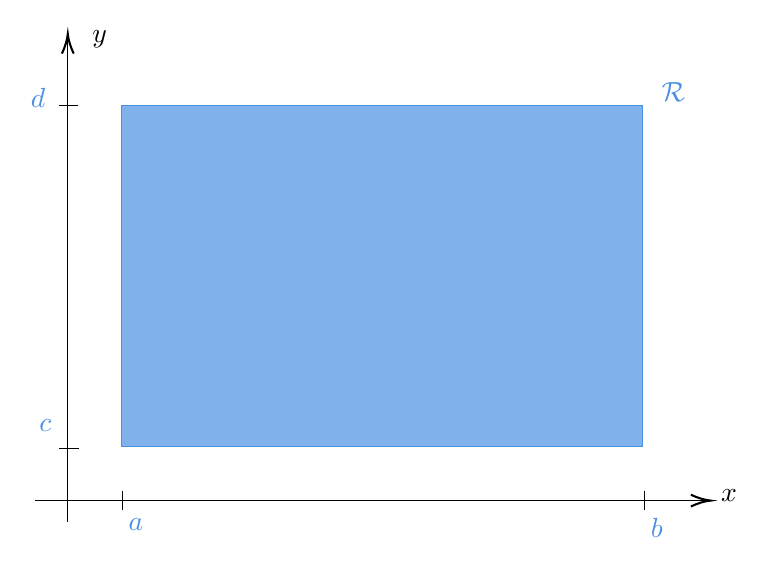
\begin{tikzpicture}[x=0.65pt,y=0.65pt,yscale=-1,xscale=1]
                %Straight Lines [id:da8996153670884857] 
                \draw    (160,281.99) -- (160,60.2) -- (160,12.55) ;
                \draw [shift={(160,10.55)}, rotate = 90] [color={rgb, 255:red, 0; green, 0; blue, 0 }  ][line width=0.75]    (10.93,-3.29) .. controls (6.95,-1.4) and (3.31,-0.3) .. (0,0) .. controls (3.31,0.3) and (6.95,1.4) .. (10.93,3.29)   ;
                %Straight Lines [id:da2832708913051102] 
                \draw    (142,270) -- (515.33,270) ;
                \draw [shift={(517.33,270)}, rotate = 180] [color={rgb, 255:red, 0; green, 0; blue, 0 }  ][line width=0.75]    (10.93,-3.29) .. controls (6.95,-1.4) and (3.31,-0.3) .. (0,0) .. controls (3.31,0.3) and (6.95,1.4) .. (10.93,3.29)   ;
                %Shape: Rectangle [id:dp7769601597656084] 
                \draw  [color={rgb, 255:red, 74; green, 144; blue, 226 }  ,draw opacity=1 ][fill={rgb, 255:red, 74; green, 144; blue, 226 }  ,fill opacity=0.7 ] (189.67,50.23) -- (479.67,50.23) -- (479.67,240) -- (189.67,240) -- cycle ;
                %Straight Lines [id:da4539992159626175] 
                \draw    (190.33,264.67) -- (190.33,275.23) ;
                %Straight Lines [id:da03805186510063541] 
                \draw    (480.67,264.43) -- (480.67,275) ;
                %Straight Lines [id:da720570136366911] 
                \draw    (166.2,241) -- (155.33,241) ;
                %Straight Lines [id:da6444573751772118] 
                \draw    (165.7,50.5) -- (154.83,50.5) ;

                % Text Node
                \draw (521.7,262.3) node [anchor=north west][inner sep=0.75pt]    {$x$};
                % Text Node
                \draw (172.2,7.4) node [anchor=north west][inner sep=0.75pt]    {$y$};
                % Text Node
                \draw (488.67,36.4) node [anchor=north west][inner sep=0.75pt]    {$\mathcal{\textcolor[rgb]{0.29,0.56,0.89}{R}}$};
                % Text Node
                \draw (192.33,278.63) node [anchor=north west][inner sep=0.75pt]    {$\textcolor[rgb]{0.29,0.56,0.89}{a}$};
                % Text Node
                \draw (482.67,278.4) node [anchor=north west][inner sep=0.75pt]    {$\textcolor[rgb]{0.29,0.56,0.89}{b}$};
                % Text Node
                \draw (142.67,223.4) node [anchor=north west][inner sep=0.75pt]    {$\textcolor[rgb]{0.29,0.56,0.89}{c}$};
                % Text Node
                \draw (138,39.4) node [anchor=north west][inner sep=0.75pt]    {$\textcolor[rgb]{0.29,0.56,0.89}{d}$};
            \end{tikzpicture}
            \caption{Região retangular \(\mathcal{R}\) no plano \(xy\)}
            \label{fig:RegiaoRetangular}
        \end{figure}
    
    Podemos mostrar (em Cálculo Avançado) que
        \begin{equation}\label{eqn.IntegralDuplaNumRetangulo}
            \int\int_\mathcal{R} f(x,y) dA = \int_a^b \left[ \int c^d f(x,y) dy \right] dx,
        \end{equation}
    em que o lado direito é uma \textit{integral iterada} que calculamos da seguinte forma:
        \begin{itemize}
            \item integramos \textit{parcialmente} em relação à variável \(y\) (supondo que \(x\) é constante) de \(c\) a \(d\), obtendo uma função de \(x\);
            \item em seguida, integramos a função obtida em relação à \(x\) de \(a\) a \(b\).
        \end{itemize}

    Mais ainda, podemos mostrar que
        \begin{equation}\label{eqn.IntegralDuplaNumRetangulo1}
            \int\int_\mathcal{R} f(x,y) dA = \int_c^d \left[ \int_a^b f(x,y) dx \right] dy.
        \end{equation}
\end{example}

As integrais iteradas que aparecem em \ref{eqn.IntegralDuplaNumRetangulo} e \ref{eqn.IntegralDuplaNumRetangulo1}, geralmente, são abreviadas da seguinte forma:
    \begin{itemize}
        \item \(\int_a^b \left[ \int_c^d f(x,y) dy \right] dx = \int_a^b \int_c^d f(x,y) dydx\)
        \item \(\int_a^b \left[ \int_c^d f(x,y) dx \right] dy = \int_a^b \int_c^d f(x,y) dxdy\)
    \end{itemize}

\begin{theorem}[Fubini]\label{thm.Fubini}\index{Teorema! Fubini}
    Se \(f\) é contínua em \[\mathcal{R} = \{(x,y) \in\R^2 : a\leq x\leq b \text{ e } c\leq y\leq d\},\] então \[\int\int_\mathcal{R} f(x,y) dA = \int_a^b \int_c^d f(x,y) dy dx = \int_c^d \int_a^b f(x,y) dxdy.\]
\end{theorem}

\begin{proof}[Ideia da prova]
    Suponha que \(f(x,y)\geq 0\) em \(\mathcal{R}\). Neste caso, a integral dupla \(\int\int_\mathcal{R} f(x,y)dA\) calcula o volume do sólido \(Q\) acima de \(\mathcal{R}\) e abaixo do gráfico \(z = f(x,y)\).
        \begin{figure}[htbp]
            \centering
            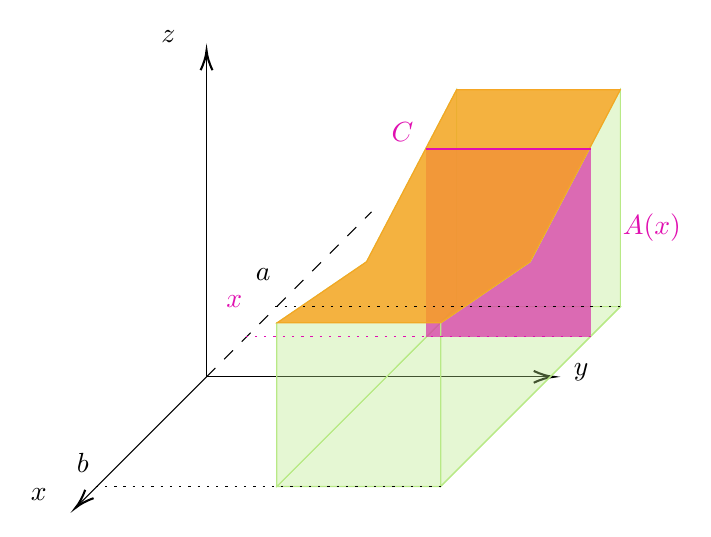
\begin{tikzpicture}[x=0.65pt,y=0.65pt,yscale=-1,xscale=1]
                %Straight Lines [id:da11678229473293145] 
                \draw    (144,205.94) -- (144,26.52) ;
                \draw [shift={(144,24.52)}, rotate = 90] [color={rgb, 255:red, 0; green, 0; blue, 0 }  ][line width=0.75]    (10.93,-3.29) .. controls (6.95,-1.4) and (3.31,-0.3) .. (0,0) .. controls (3.31,0.3) and (6.95,1.4) .. (10.93,3.29)   ;
                %Straight Lines [id:da41024481908543386] 
                \draw    (144,205.94) -- (334.83,205.94) ;
                \draw [shift={(336.83,205.94)}, rotate = 180] [color={rgb, 255:red, 0; green, 0; blue, 0 }  ][line width=0.75]    (10.93,-3.29) .. controls (6.95,-1.4) and (3.31,-0.3) .. (0,0) .. controls (3.31,0.3) and (6.95,1.4) .. (10.93,3.29)   ;
                %Straight Lines [id:da14381184794254986] 
                \draw    (144,205.94) -- (72.55,277.39) ;
                \draw [shift={(71.13,278.81)}, rotate = 315] [color={rgb, 255:red, 0; green, 0; blue, 0 }  ][line width=0.75]    (10.93,-3.29) .. controls (6.95,-1.4) and (3.31,-0.3) .. (0,0) .. controls (3.31,0.3) and (6.95,1.4) .. (10.93,3.29)   ;
                %Straight Lines [id:da11136546916048007] 
                \draw  [dash pattern={on 4.5pt off 4.5pt}]  (144,205.94) -- (235.7,114.24) ;
                %Shape: Polygon [id:ds05009258866603372] 
                \draw  [color={rgb, 255:red, 184; green, 233; blue, 134 }  ,draw opacity=1 ][fill={rgb, 255:red, 184; green, 233; blue, 134 }  ,fill opacity=0.2 ] (282.99,46.35) -- (282.99,166.92) -- (183.13,266.9) -- (183.13,175.98) -- (232.94,141.97) -- cycle ;
                %Shape: Rectangle [id:dp04988373310574079] 
                \draw  [color={rgb, 255:red, 184; green, 233; blue, 134 }  ,draw opacity=1 ][fill={rgb, 255:red, 184; green, 233; blue, 134 }  ,fill opacity=0.2 ] (283.12,166.92) -- (374.03,166.92) -- (274.05,266.9) -- (183.13,266.9) -- cycle ;
                %Shape: Rectangle [id:dp03272205490850577] 
                \draw  [color={rgb, 255:red, 184; green, 233; blue, 134 }  ,draw opacity=1 ][fill={rgb, 255:red, 184; green, 233; blue, 134 }  ,fill opacity=0.2 ] (282.99,46.35) -- (374.03,46.35) -- (374.03,166.92) -- (282.99,166.92) -- cycle ;
                %Shape: Rectangle [id:dp018441446147018592] 
                \draw  [draw opacity=0][fill={rgb, 255:red, 224; green, 16; blue, 177 }  ,fill opacity=0.75 ] (266.2,79.28) -- (357.66,79.28) -- (357.66,183.55) -- (266.2,183.55) -- cycle ;
                %Shape: Rectangle [id:dp4455586741976165] 
                \draw  [color={rgb, 255:red, 184; green, 233; blue, 134 }  ,draw opacity=1 ][fill={rgb, 255:red, 184; green, 233; blue, 134 }  ,fill opacity=0.2 ] (183.13,175.98) -- (274.18,175.98) -- (274.18,266.9) -- (183.13,266.9) -- cycle ;
                %Shape: Polygon [id:ds3649260996398733] 
                \draw  [color={rgb, 255:red, 184; green, 233; blue, 134 }  ,draw opacity=1 ][fill={rgb, 255:red, 184; green, 233; blue, 134 }  ,fill opacity=0.2 ] (374.03,46.35) -- (374.03,166.92) -- (274.18,266.9) -- (274.18,175.98) -- (323.98,141.97) -- cycle ;
                %Shape: Polygon [id:ds09490738366832097] 
                \draw  [color={rgb, 255:red, 245; green, 166; blue, 35 }  ,draw opacity=1 ][fill={rgb, 255:red, 245; green, 166; blue, 35 }  ,fill opacity=0.85 ] (374.03,46.35) -- (323.85,141.97) -- (274.18,175.98) -- (183.13,175.98) -- (232.94,141.97) -- (282.99,46.35) -- cycle ;
                %Straight Lines [id:da2016852206431038] 
                \draw [color={rgb, 255:red, 224; green, 16; blue, 177 }  ,draw opacity=1 ] [dash pattern={on 0.84pt off 2.51pt}]  (165.7,183.55) -- (357.7,183.55) ;
                %Straight Lines [id:da4489938492590413] 
                \draw  [dash pattern={on 0.84pt off 2.51pt}]  (182.2,166.92) -- (374.03,166.92) ;
                %Straight Lines [id:da5996164254690274] 
                \draw  [dash pattern={on 0.84pt off 2.51pt}]  (82.35,266.9) -- (274.18,266.9) ;
                %Straight Lines [id:da5316237939610688] 
                \draw [color={rgb, 255:red, 224; green, 16; blue, 177 }  ,draw opacity=1 ]   (266.2,79.28) -- (357.66,79.28) ;

                % Text Node
                \draw (44.87,266.73) node [anchor=north west][inner sep=0.75pt]  [font=\normalsize]  {$x$};
                % Text Node
                \draw (117.43,12.14) node [anchor=north west][inner sep=0.75pt]  [font=\normalsize]  {$z$};
                % Text Node
                \draw (346.7,197.03) node [anchor=north west][inner sep=0.75pt]  [font=\normalsize]  {$y$};
                % Text Node
                \draw (153.5,159.1) node [anchor=north west][inner sep=0.75pt]  [color={rgb, 255:red, 224; green, 16; blue, 177 }  ,opacity=1 ]  {$x$};
                % Text Node
                \draw (374,114.07) node [anchor=north west][inner sep=0.75pt]    {$\textcolor[rgb]{0.88,0.06,0.69}{A( x)}$};
                % Text Node
                \draw (170,144.1) node [anchor=north west][inner sep=0.75pt]    {$a$};
                % Text Node
                \draw (70.5,247.1) node [anchor=north west][inner sep=0.75pt]    {$b$};
                % Text Node
                \draw (245.5,63.1) node [anchor=north west][inner sep=0.75pt]  [color={rgb, 255:red, 224; green, 16; blue, 177 }  ,opacity=1 ]  {$C$};
            \end{tikzpicture}
            \caption{Área abaixo da curva \(C\) e acima da região \(\mathcal{R}\)}
            \label{fig:AreaAbaixodaCurva}
        \end{figure}

    Da teoria de integral definida para funções de uma variável, podemos calcular o volume de \(Q\) fazendo \[V = \int_a^b A(x) dx,\] no qual \(A(x)\) é a área da seção transversal de \(Q\) como acima.

    Agora, note que \(A(x)\) é a área abaixo da curva \(C\) que tem equação \(z = f(x,y)\), com \(x\) constante e \(c\leq y\leq d\). Logo \[A(x) = \int_c^d f(x,y) dy.\] Assim \[\int\int_\mathcal{R} f(x,y) dA = V = \int_a^b A(x) dx = \int_a^b \int_c^d f(x,y) dydx.\]
\end{proof}

Em geral, se \(\mathcal{R}\) é uma região \(\mathcal{R}_x\) ou \(\mathcal{R}_y\), como abaixo, ainda podemos definir uma integral dupla iterada.
    \begin{figure}[htbp]
            \centering
            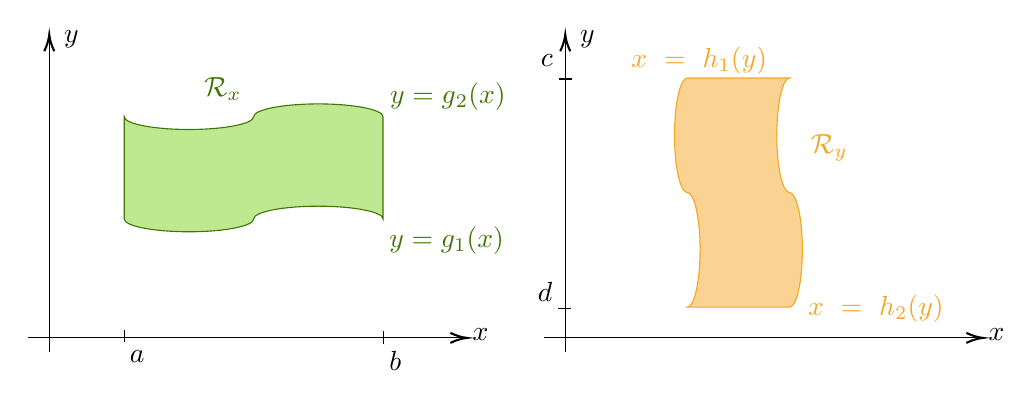
\begin{tikzpicture}[x=0.55pt,y=0.55pt,yscale=-1,xscale=1]
                %Straight Lines [id:da09127950708327948] 
                \draw    (33.02,239.49) -- (33.02,69.15) -- (33.02,33.01) ;
                \draw [shift={(33.02,31.01)}, rotate = 90] [color={rgb, 255:red, 0; green, 0; blue, 0 }  ][line width=0.75]    (10.93,-3.29) .. controls (6.95,-1.4) and (3.31,-0.3) .. (0,0) .. controls (3.31,0.3) and (6.95,1.4) .. (10.93,3.29)   ;
                %Straight Lines [id:da773781962025611] 
                \draw    (19.2,230.28) -- (305.47,230.28) ;
                \draw [shift={(307.47,230.28)}, rotate = 180] [color={rgb, 255:red, 0; green, 0; blue, 0 }  ][line width=0.75]    (10.93,-3.29) .. controls (6.95,-1.4) and (3.31,-0.3) .. (0,0) .. controls (3.31,0.3) and (6.95,1.4) .. (10.93,3.29)   ;
                %Straight Lines [id:da22603710536428145] 
                \draw    (82.32,225.19) -- (82.32,233.3) ;
                %Straight Lines [id:da0410279420552665] 
                \draw    (252.81,226.01) -- (252.81,234.12) ;
                %Straight Lines [id:da2181270381656647] 
                \draw    (372.02,239.49) -- (372.02,69.15) -- (372.02,33.01) ;
                \draw [shift={(372.02,31.01)}, rotate = 90] [color={rgb, 255:red, 0; green, 0; blue, 0 }  ][line width=0.75]    (10.93,-3.29) .. controls (6.95,-1.4) and (3.31,-0.3) .. (0,0) .. controls (3.31,0.3) and (6.95,1.4) .. (10.93,3.29)   ;
                %Straight Lines [id:da8283285342869068] 
                \draw    (358.2,230.28) -- (644.47,230.28) ;
                \draw [shift={(646.47,230.28)}, rotate = 180] [color={rgb, 255:red, 0; green, 0; blue, 0 }  ][line width=0.75]    (10.93,-3.29) .. controls (6.95,-1.4) and (3.31,-0.3) .. (0,0) .. controls (3.31,0.3) and (6.95,1.4) .. (10.93,3.29)   ;
                %Straight Lines [id:da4011344083802706] 
                \draw    (375.79,211.01) -- (367.44,211.01) ;
                %Straight Lines [id:da7849663867312362] 
                \draw    (376.4,60.2) -- (368.06,60.2) ;
                %Flowchart: Punched Tape [id:dp4996860470719555] 
                \draw  [color={rgb, 255:red, 65; green, 117; blue, 5 }  ,draw opacity=1 ][fill={rgb, 255:red, 126; green, 211; blue, 33 }  ,fill opacity=0.5 ] (82.3,84.95) .. controls (82.3,89.59) and (101.33,93.35) .. (124.8,93.35) .. controls (148.27,93.35) and (167.3,89.59) .. (167.3,84.95) .. controls (167.3,80.31) and (186.33,76.55) .. (209.8,76.55) .. controls (233.27,76.55) and (252.3,80.31) .. (252.3,84.95) -- (252.3,152.15) .. controls (252.3,147.51) and (233.27,143.75) .. (209.8,143.75) .. controls (186.33,143.75) and (167.3,147.51) .. (167.3,152.15) .. controls (167.3,156.79) and (148.27,160.55) .. (124.8,160.55) .. controls (101.33,160.55) and (82.3,156.79) .. (82.3,152.15) -- cycle ;
                %Flowchart: Punched Tape [id:dp7633494337486438] 
                \draw  [color={rgb, 255:red, 245; green, 166; blue, 35 }  ,draw opacity=1 ][fill={rgb, 255:red, 245; green, 166; blue, 35 }  ,fill opacity=0.5 ] (519.4,59.55) .. controls (514.76,59.55) and (511,76.4) .. (511,97.17) .. controls (511,117.95) and (514.76,134.8) .. (519.4,134.8) .. controls (524.04,134.8) and (527.8,151.65) .. (527.8,172.42) .. controls (527.8,193.2) and (524.04,210.05) .. (519.4,210.05) -- (452.2,210.05) .. controls (456.84,210.05) and (460.6,193.2) .. (460.6,172.42) .. controls (460.6,151.65) and (456.84,134.8) .. (452.2,134.8) .. controls (447.56,134.8) and (443.8,117.95) .. (443.8,97.17) .. controls (443.8,76.4) and (447.56,59.55) .. (452.2,59.55) -- cycle ;

                % Text Node
                \draw (309.43,222.6) node [anchor=north west][inner sep=0.75pt]    {$x$};
                % Text Node
                \draw (41,26.83) node [anchor=north west][inner sep=0.75pt]    {$y$};
                % Text Node
                \draw (648.43,222.6) node [anchor=north west][inner sep=0.75pt]    {$x$};
                % Text Node
                \draw (380,26.83) node [anchor=north west][inner sep=0.75pt]    {$y$};
                % Text Node
                \draw (84.32,236.7) node [anchor=north west][inner sep=0.75pt]    {$a$};
                % Text Node
                \draw (254.81,237.52) node [anchor=north west][inner sep=0.75pt]    {$b$};
                % Text Node
                \draw (254.8,155.55) node [anchor=north west][inner sep=0.75pt]    {$\textcolor[rgb]{0.25,0.46,0.02}{y=g_{1}( x)}$};
                % Text Node
                \draw (255.3,60.95) node [anchor=north west][inner sep=0.75pt]    {$\textcolor[rgb]{0.25,0.46,0.02}{y=g}\textcolor[rgb]{0.25,0.46,0.02}{_{2}}\textcolor[rgb]{0.25,0.46,0.02}{(}\textcolor[rgb]{0.25,0.46,0.02}{x}\textcolor[rgb]{0.25,0.46,0.02}{)}$};
                % Text Node
                \draw (354.31,42.2) node [anchor=north west][inner sep=0.75pt]    {$c$};
                % Text Node
                \draw (352.31,192.2) node [anchor=north west][inner sep=0.75pt]    {$d$};
                % Text Node
                \draw (413.8,37.4) node [anchor=north west][inner sep=0.75pt]    {$\textcolor[rgb]{0.96,0.65,0.14}{x\ =\ h_{1}( y)}$};
                % Text Node
                \draw (529.8,200.4) node [anchor=north west][inner sep=0.75pt]    {$\textcolor[rgb]{0.96,0.65,0.14}{x\ =\ h}\textcolor[rgb]{0.96,0.65,0.14}{_{2}}\textcolor[rgb]{0.96,0.65,0.14}{(}\textcolor[rgb]{0.96,0.65,0.14}{y}\textcolor[rgb]{0.96,0.65,0.14}{)}$};
                % Text Node
                \draw (133,57.4) node [anchor=north west][inner sep=0.75pt]    {$\textcolor[rgb]{0.25,0.46,0.02}{\mathcal{R}_{x}}$};
                % Text Node
                \draw (531.67,94.73) node [anchor=north west][inner sep=0.75pt]    {$\textcolor[rgb]{0.96,0.65,0.14}{\mathcal{R}_{y}}$};
            \end{tikzpicture}
            \caption{Regiões do tipo \(\mathcal{R}_x\) e \(\mathcal{R}_y\)}
            \label{fig:RegioesTipoRxRy}
        \end{figure}


\begin{definition}[Integrais iteradas]\index{Integrais iteradas}
    Para as regiões \(\mathcal{R}_x\) e \(\mathcal{R}_y\) acima temos
        \begin{enumerate}
            \item \[\int_a^b \int_{g_1(x)}^{g_2(x)} f(x,y) dy dx = \int_a^b \left[ \int_{g_1(x)}^{g_2(x)} dy \right] dx.\]
            \item \[\int_c^d \int_{h_1(x)}^{h_2(x)} f(x,y) dx dy = \int_c^d \left[ \int_{h_1(y)}^{h_2(y)} dx \right] dy.\]
        \end{enumerate}
\end{definition}

\begin{example}
    Calcule \[\int_1^4 \int_{-1}^2 (2x + 6x^2y) dy dx.\]

    {\cv FIGURA}

    Temos
        \begin{align*}
            \int_1^4 \int_{-1}^2 (2x + 6x^2y) dy dx
                & = \int_1^4 \left( 2xy + 6x^2\frac{y^2}{2} \right)\bigg|_{-1}^2 dx \\
                & = \int_1^4 4x + 12x^2 - (-2x + 3x^2) dx \\
                & = \int_1^4 6x + 9x^2 dx \\
                & = \left( 6\frac{x^2}{2} + 9\frac{x^3}{3} \right)\bigg|_1^4 = 234.
        \end{align*}
\end{example}

\begin{exercise}
    Calcule \(\int_{-1}^2 \int_1^4 (2x + 6x^2) dxdy\).
\end{exercise}

\begin{example}
    Calcule \(\int_0^2 \int_{x^2}^{2x} (x^3 + 4y) dy dx\).

    {\cv FIGURA}

    Temos
        \begin{align*}
            \int_0^2 \int_{x^2}^{2x} (x^3 + 4y) dy dx
                & = \int_0^2 \left( x^3 y + \frac{4y^2}{2} \right)\bigg|_{x^2}^{2x} dx \\
                & = \int_0^2 \left[ \left( x^3\cdot 2x + 4\frac{(2x)^2}{2} \right) - \left( x^3\cdot x^2 + 4\frac{(x^2)^2}{2} \right) \right] dx \\
                & = \int_0^2 2x^4 + 8x^2 - x^5 - 2x^4 dx \\
                & = \int_0^2 8x^2 - x^5 dx \\
                & = \left( \frac{8x^3}{3} - \frac{x^6}{6} \right)\bigg|_0^2 = \frac{32}{3} 
        \end{align*}
\end{example}

\begin{example}
    Calcule \(\int_1^3 \int_{\frac{\pi}{6}}^{y^2} 2y\cdot \cos(x) dxdy\).
        {\cv FIGURA}

    Temos \(h_1(y) = \frac{\pi}{6}\) e \(h_2(y) = y^2\). A interseção de \(h_1\) e \(h_2\) ocorre quando \(y^2 = \frac{\pi}{6}\), ou seja, \(y = \pm \sqrt{\frac{\pi}{6}}\), porém, sendo \(y>0\), a interseção ocorre apenas quando \(y = \sqrt{\frac{\pi}{6}}\).

    Do anterior,
        \begin{align*}
            \int_1^3 \int_{\frac{\pi}{6}}^{y^2} 2y\cdot\cos(x) dx dy
                & = \int_1^3 (2y\sin(x))\bigg|_{\frac{\pi}{6}}^{y^2} dy \\
                & = \int_1^3 2y\sin(y^2) - 2y\sin\left( \frac{\pi}{6} \right) dy \\
                & = \int_1^3 2y\sin(y^2) - y dy \\
                & = \int_1^9 \sin(u) du - \frac{y^2}{2}\bigg|_1^3 \\
                & = -\cos(u)\bigg|_1^9 - \frac{9}{2} + \frac{1}{2} \\
                & = \cos(1) - \cos(9) - 4
        \end{align*}

\end{example}

A seguir apresentaremos um resultado que generaliza o Teorema de Fubini \ref{thm.Fubini} para o caso de regiões \(\mathcal{R}_x\) e \(\mathcal{R}_y\).

\begin{theorem}[Fubini]\index{Teorema!Fubini}\label{thm.Fubini1}
    Seja \(f(x,y)\) contínua numa região \(\mathcal{R}\).
        \begin{enumerate}
            \item Numa região \(\mathcal{R}_x\), vale \[\int\int_{\mathcal{R}_x} f(x,y) dA = \int_a^b \int_{g_1(x)}^{g_2(x)} f(x,y) dy dx.\]
            \item Numa região \(\mathcal{R}_y\), \[\int\int_{\mathcal{R}_y} f(x,y) dA = \int_c^d \int_{h_1(y)}^{h_2(y)} f(x,y) dx dy.\]
        \end{enumerate}
\end{theorem}

\begin{proof}[Ideia da prova]
    Suponha que \(f(x,y) \geq 0\), para todo \((x,y)\in\mathcal{R}_x\) e denote por \(S\) o gráfico de \(f\), \(Q\) o sólido sob \(S\) e sobre \(\mathcal{R}_x\) e \(V\) o volume de \(Q\).

    Neste caso, sabemos que \[\int\int_{\mathcal{R}_x} f(x,y) dA = V.\]
        {\cv FIGURA}
    
    Da teoria de integrais definidas para funções de uma variável, uma fórmula para calcular o volume de \(Q\) é \[V = \int_a^b A(x) dx\] no qual \(A(x)\) é a área da seção transversal de \(Q\), como na figura.

    Por outro lado, \(A(x)\) é a área abaixo da curva \(C\) que tem equação \(z = f(x,y)\), com \(x\) constante e \(g_1(x) \leq y \leq g_2(x)\).

    Logo \[A(x) = \int_{g_1(x)}^{g_2(x)} f(x,y) dy,\] portanto \[\int\int_{\mathcal{R}_x} = \int_a^b A(x) dx = \int_a^b \int_{g_1(x)}^{g_2(x)} f(x,y) dydx.\]
\end{proof}

\begin{remark}
    Se \(\mathcal{R}\) é uma região mais complicada, podemos tentar dividir \(\mathcal{R}\) em subregiões \(\mathcal{R}_x\) e \(\mathcal{R}_y\), aplicar o Teorema \ref{thm.Fubini1} em cada uma e somar os valores das integrais resultantes.
\end{remark}

\begin{remark}
    Para o cálculo de integrais duplas é importante fazer um esboço da região \(\mathcal{R}\) e determinar suas fronteiras.
\end{remark}

\begin{example}
    Seja \(\mathcal{R}\) a região no plano-xy limitado pelos gráficos de \(y = x^2\) e \(y=2x\). Calcule \(\int\int_\mathcal{R} (x^3 + 4y) dA.\)

    Começamos fazendo um esboço da região \(\mathcal{R}\).

    \textbf{\textit{Interseção: }} Note que \[x^2 = 2x \Rightarrow x^2 - 2x =0 \Rightarrow x(x-2) =0 \Rightarrow \begin{cases}
        x=0 \\
        x=2
    \end{cases}.\]
        {\cv FIGURA}

    Note que \(f(x,y) = x^3 + 4y\) é contínua em \(\mathcal{R}\).

    Se consideramos \(\mathcal{R} = \mathcal{R}_x\), com \(0\leq x \leq 2\) e \(x^2 \leq y \leq 2x\), então
        \begin{align*}
            \int\int_\mathcal{R} (x^3 + 4y) dA
                & = \int_0^2 \int_{x^2}^{2x} (x^3 + 4y) dy dx \\
                & = \int_0^2 \left( x^3 y + 4\left( \frac{y^2}{2} \right) \right)\bigg|_{x^2}^{2x} dx \\
                & = \int_0^2 x^3\cdot 2x + 2(2x)^2 - x^3\cdot x^2 - 2(x^2)^2 dx \\
                & = \int_0^2 8x^2 - x^5 dx \\
                & = \left( 8\frac{x^3}{3} - \frac{x^6}{6} \right)\bigg|_0^2 = \frac{32}{3}
        \end{align*}

    Agora, se consideramos \(\mathcal{R} = \mathcal{R}_y\), com \(0\leq y\leq 4\) e \(\frac{y}{2} \leq x \leq \sqrt{y}\), então \[\int\int_\mathcal{R} x^3 + 4y dA = \int_0^4 \int_{\frac{y}{2}}^{\sqrt{y}} x^3 + 4y dx dy = \frac{32}{3}.\]
\end{example}

\begin{example}
    Seja \(\mathcal{R}\) a região limitada pelos gráficos de \(y = \sqrt{x}\), \(y = \sqrt{3x - 18}\) e \(y=0\). Se \(f\) é uma função contínua qualquer em \(\mathcal{R}\), expresse a integral dupla de \(f\) em \(\mathcal{R}\) em termos de integrais iteradas.

    Analisemos a interseção entre \(y = \sqrt{x}\) e \(y = \sqrt{3x-18}\). Temos que \[\sqrt{x} = \sqrt{3x - 18} \Rightarrow x = 3x - 18 \Rightarrow x=9\]
    {\cv FIGRURA}

    Se olhamos \(\mathcal{R} = \mathcal{R}_1\cup\mathcal{R}_2\), com \[\mathcal{R}_1 = \mathcal{R}_{1,x} = \{(x,y)\in\R^2 : 0\leq x\leq 6 \text{ e } 0\leq y\leq \sqrt{x}\}\] \[\mathcal{R}_2 = \mathcal{R}_{2,x} = \{(x,y)\in\R^2 : 6\leq x \leq 9 \text{ e } \sqrt{3x-18}\leq y\leq \sqrt{x}\}.\]

    Logo
        \begin{align*}
            \int\int_\mathcal{R} 
                & = f(x,y) dA \\
                & = \int\int_{\mathcal{R}_1} f(x,y) dA + \int\int_{\mathcal{R}_2} f(x,y) dA \\
                & = \int_0^6\int_0^{\sqrt{x}} f(x,y) dydx + \int_6^9\int_{\sqrt{3x-18}}^{\sqrt{x}} f(x,y) dy dx.
        \end{align*}

    Também podemos olhar \(\mathcal{R} = \mathcal{R}_y\), com \[\mathcal{R}_y = \{(x,y)\in\R^2 : 0 \leq y \leq 3 \text{ e } y^2 \leq x \leq \frac{y^2}{2} + 6\}.\]

    Logo, \[\int\int_\mathcal{R} f(x,y) dA = \int_0^3 \int_{y^2}^{\frac{y^2}{2}+6} f(x,y) dxdy.\]
\end{example}

\begin{remark}
    Se \(\mathcal{R} = \mathcal{R}_x\) e \(\mathcal{R} = \mathcal{R}_y\) e \(f\) é contínua em \(\mathcal{R}\), pelo Teorema \ref{thm.Fubini1}, a ordem de integração é indiferente, como vimos nos exemplos acima. Porém, às vezes, pode ser muito difícil, ou mesmo impossível, calcular uma integral dupla iterada, mas, invertendo a ordem de integração, pode-se chegar a uma integral equivalente que pode ser calculada com facilidade.

    \textbf{Conclusão: } Se \(\mathcal{R} = \mathcal{R}_x = \mathcal{R}_y\) e \(f\) é contínua em \(\mathcal{R}\), a ordem de integração pode ser escolhida, dependendo da dificuldade que encontramos na integração de \(f\) em \(\mathcal{R}_x\) ou \(\mathcal{R}_y\).
\end{remark}

\begin{example}
    Calcule \(\int_0^4 \int_{\sqrt{y}}^{2} y\cos(x^5) dxdy\).

    Note que, pela integral dada, temos a região \[\mathcal{R} = \mathcal{R}_y = \{(x,y)\in\R^2 : 0\leq y\leq 4 \text{ e } \sqrt{y}\leq x\leq 2\}\]
        {\cv FIGURA}

    Agora, a integral \[\int_0^4 \int_{\sqrt{y}}^{2} y\cos(x^5) dxdy\] não parece ser fácil de ser calculada. No entanto, observando \(\mathcal{R}\) com \(\mathcal{R}_x\) temos \[\mathcal{R} = \mathcal{R}_x = \{(x,y)\in\R^2 : 0\leq x\leq 2 \text{ e } 0\leq y\leq x^2 \}\] e \[\int_0^4 \int_{\sqrt{y}}^2 y\cos(x^5) dxdy = \int_0^2 \int_0^{x^2} y \cos(x^5) dy dx = \int_0^2 cos(x^5)\cdot \frac{x^4}{2} dx\]
\end{example}



% \section{Integrais duplas em coordenadas polares}

% \section{Integrais triplas}

% \section{Integrais triplas em coordenadas cilíndricas}

% \section{Integrais triplas em coordenadas esféricas}

% \section{Mudança de variáveis e jacobianos}